% !TeX encoding = UTF-8
% !TeX spellcheck = pt_BR
% ------------------------------------------------------------------
% ------------------------------------------------------------------
% ICMC: Modelo de Trabalho Acadêmico (tese de doutorado, dissertação de
% mestrado e trabalhos monográficos em geral) em conformidade com
% ABNT NBR 14724:2011: Informação e documentação - Trabalhos acadêmicos -
% Apresentação
% ------------------------------------------------------------------
% -----------------------------------------------------------------

% Opções:
%   Qualificação         = qualificacao
%   Curso                = doutorado/mestrado
%   Situação do trabalho = pre-defesa/pos-defesa (exceto para qualificação)
% -- opções do pacote babel --
% Idioma padrão = brazil
    %spanish,           % idioma adicional para hifenização
    %english,           % idioma adicional para hifenização
    %brazil             % o último idioma é o principal do documento
%\documentclass[mestrado, pos-defesa, spanish, english, brazil]{packages/icmc}

\documentclass[mestrado, pre-defesa, english, brazil]{packages/icmc}
%\documentclass[draft,mestrado, pre-defesa, english, brazil]{packages/icmc}

%%%%%%%%%%

\usepackage[utf8]{inputenc} % codificação de entrada e fontes
\usepackage[T1]{fontenc}
%\usepackage[pdftex]{color,graphicx} % incluir gráficos
\usepackage{multirow} % tabela partida em duas
\usepackage{indentfirst} % indenta o primeiro parágrafo de cada seção.
\usepackage{microtype} % melhor o espaço entre as palavras

%%%%%%%%%%

% ---
% Pacotes Opcionais
% ---
\usepackage{rotating} % Usado para rotacionar o texto
\usepackage[all,knot,arc,import,poly]{xy} % Pacote para desenhos gráficos
% Este pacote pode conflitar com outros pacotes gráficos como o ``pictex''
% Então é necessário usar apenas um dos pacotes conflitantes

\newcommand{\VerbL}{0.52\textwidth}
\newcommand{\LatL}{0.42\textwidth}

% Colorinlistoftodos package: to insert colored comments so authors can collaborate on the content.
% Link: http://www.inf.ufes.br/~vitorsouza/blog/controle-de-alteracoes-em-latex-usando-git-e-sourcetree/
\usepackage[colorinlistoftodos, textwidth=20mm, textsize=footnotesize]{todonotes}
\newcommand{\ideia}[1]{\todo[author=\textbf{Ideia},color=green!30,caption={},inline]{#1}}
\newcommand{\duvida}[1]{\todo[author=\textbf{Dúvida},color=red!30,caption={},inline]{#1}}

% ---
% Informações de dados para CAPA e FOLHA DE ROSTO
% ---
% Tanto na capa quanto nas folhas de rosto apenas a primeira letra da primeira palavra (ou nomes próprios) devem estar em letra maiúscula, todas as demais devem ser em letra minúscula.
\tituloPT{Otimização do encaminhamento de mensagens oportunistas em VANETs baseada na categorização de veículos}
\tituloEN{Vehicular mobility habits evaluation to optimize message routing opportunists in VANETs}
\autor[Ribeiro, J. B.]{João Batista Ribeiro}
\genero{M} % Gênero do autor (M = Masculino / F = Feminino)
\orientador[Orientador]{Prof. Dr.}{Edson dos Santos Moreira}
%\coorientador{Prof. Dr.}{Fulano de Tal}
\curso{CCMC}
\data{20}{02}{2017} % Data do depósito
% ---

% ---
% RESUMOS
% ---

% Resumo em PORTUGUÊS
% conter no máximo 500 palavras
% conter no mínimo 1 e no máximo 5 palavras-chave
\textoresumo[brazil]{
    A quantidade de veículos aumenta a cada dia e aliada com a falta de infraestrutura necessária, torna a situação do trânsito mundial ainda mais caótica e perigosa. Esse cenário pode ser melhorado com as VANETs (\textit{Vehicular Ad hoc NETworks}) que, aliadas aos Sistemas de Transporte Inteligente, tem o objetivo de melhorar a eficiência, a segurança e o conforto dos passageiros nos sistemas de transporte. Para tal, as VANETs utilizam interfaces de comunicação sem fio e sensores implantados nos veículos. Os veículos pertencentes a uma VANET podem se comunicar entre si ou com uma infraestrutura, que é assumida a ser localizada na margem da estrada. A comunicação nas VANETs é feita por meio de encontros oportunistas, assim uma mensagem pode passar por um ou vários nós intermediários até chegar ao nó de destino. Para rotear estas mensagens, foram desenvolvidos alguns protocolos. Neste projeto esperamos classificar os veículos em categorias em função dos seus hábitos de mobilidade e assim criar uma maneira de se inferir o padrão de mobilidade dos veículos de forma prática. Em sequência incorporá-la em algum protocolo de roteamento, assim como seus hábitos de mobilidade, com o intuito de melhorar o encaminhamento de mensagens nas VANETs. Os resultados serão validados por meio de simulações.

    \textcolor{red}{Dissertação - versão 2}

    }{Vehicular Ad hoc Networks, Encaminhamento de Mensagens, Redes Oportunistas, Sistemas de Transporte Inteligente}

% resumo em INGLÊS
% conter no máximo 500 palavras
% conter no mínimo 1 e no máximo 5 palavras-chave
\textoresumo[english]{
    The number of vehicles is increasing daily and combined with the lack of necessary infrastructure, makes the situation of the global traffic even more chaotic and dangerous. This scenario can be improved with VANETs (Vehicular Ad hoc Networks) which, combined with the Intelligent Transport Systems, aims to improve the efficiency, safety and passenger comfort in transport systems. To this end, VANETs use wireless communication interfaces and sensors deployed in vehicles. Vehicles belonging to a VANET can communicate with each other or with an infrastructure, which is assumed to be located on the side of the road. The communication in VANETs is made through opportunistic encounters, so a message can pass through one or more intermediate nodes until you reach your destination. To route these messages were developed some algorithms. In this project we hope to classify vehicles into categories according to their mobility habits and thus create a way to infer the pattern of mobility of practical vehicles. In consequently insert a routing algorithm classification of vehicles, as well as their mobility habits, in order to improve the routing of messages in VANETs. The results will be validated by simulations.
    }{Vehicular Ad hoc Networks, Message Forwarding, Opportunistic Networks, Intelligent Transportation Systems}

% ---
% Configurações de aparência do PDF final
% ---
\hypersetup{
    colorlinks=true % false: boxed links; true: colored links
}
% ---

% ----------------------------------------------------------
% ELEMENTOS PRÉ-TEXTUAIS
% ----------------------------------------------------------

% Inserir a ficha catalográfica
%\incluifichacatalografica*{tex/fichaCatalografica.pdf}
%\incluifichacatalografica{634} % Código Cutter: número atribuído ao sobrenome do autor. Para obtê-lo, consulte a tabela Cutter Sanborn (em http://203.241.185.12/asd/board/Author/upfile/abcd.htm), procure pelo sobrenome ou forma mais próxima ao sobrenome completo e coloque o número indicado como parâmetro.
\incluifichacatalografica{333}

% DEDICATÓRIA / AGRADECIMENTO / EPÍGRAFE
\textodedicatoria*{tex/pre-textual/dedicatoria}
\textoagradecimentos*{tex/pre-textual/agradecimentos}
\textoepigrafe*{tex/pre-textual/epigrafe}

% Inclui a lista de figuras
\incluilistadefiguras

% Inclui a lista de tabelas
\incluilistadetabelas

% Inclui a lista de quadros
%\incluilistadequadros

% Inclui a lista de algoritmos
%\incluilistadealgoritmos

% Inclui a lista de códigos
%\incluilistadecodigos

% Inclui a lista de siglas e abreviaturas
\incluilistadesiglas

% Inclui a lista de símbolos
%\incluilistadesimbolos

% ----
% Início do documento
% ----
\begin{document}
% ----------------------------------------------------------
% ELEMENTOS TEXTUAIS
% ----------------------------------------------------------
\textual

%\chapter{Introdução}
%\label{chapter:introducao}
%% Comando simples para exibir comandos Latex no texto
\newcommand{\comando}[1]{\textbf{$\backslash$#1}}

Este documento explica brevemente como trabalhar com a classe \LaTeX~\textit{icmc} para confeccionar trabalhos acadêmicos seguindo as normas da \sigla{ABNT}{Associação Brasileira de Normas Técnicas} e as \aspas{\textit{Diretrizes para apresentação de dissertações e teses da USP: documento eletrônico e impresso. Parte I (ABNT)}}, publicado pelo \sigla{SIBi}{Sistema Integrado de Bibliotecas} USP. O presente manual também atende as exigências prevista no regimento do Programa de Pós-graduação em \sigla{CCMC}{Ciências da Computação e Matemática Computacional} do \sigla{ICMC}{Instituto de Ciências Matemáticas e de Computação} da \sigla{USP}{Universidade de São Paulo}.


A classe \textit{icmc} foi construída com base na última versão da classe \textit{abntex2} e do pacote \textit{abntex2cite}. Portanto, este documento exemplifica a elaboração de trabalho
acadêmico (tese, dissertação e outros do gênero) produzido conforme a ABNT NBR
14724:2011 \textit{Informação e documentação - Trabalhos acadêmicos - Apresentação}.

Assim, é altamente recomendável que seja consultada a documentação do \textit{abntex2}\footnote{https://code.google.com/p/abntex2/downloads/list}. A classe \textit{abntex2} foi desenvolvida para facilitar a escrita de documentos seguindo as normas da ABNT no ambiente \LaTeX\;\cite{frasson:2005:classe_abnt}.

Todo o trabalho de pesquisa e ajustes da presente classe \LaTeX~\emph{icmc} foram feitos pelo aluno mestrado do Programa de Pós-graduação em Ciência da Computação e Matemática Computacional, Humberto Lidio Antonelli, durante a confecção da sua monografia de qualificação.

O requisito básico para utilização da classe \textit{icmc} é criar um documento desta classe com o comando
\comando{documentclass[@parameters]\{icmc\}} e ter, no diretório de trabalho, o arquivo \emph{icmc.cls} presente. Entretanto, recomenda-se fortemente manter a estrutura de diretório inicial fornecida por este modelo. Além disso, para que o documento esteja em conformidade com as normas exigidas pelo programa de Pós-Graduação, o \textbf{projeto deve ser compilado utilizando \textit{XeLaTeX} ou \textit{LuaLaTeX}}. Esse processo de compilação é necessário para que as fontes externas utilizadas para gerar a capa sejam incluídas.

Os parâmetros possíveis utilizados pelo \comando{documentclass} são:
\begin{description}
\item[qualificacao] Exclusivamente para monografias de qualificação em geral;
\item[mestrado / doutorado] Identifica o curso ao qual o aluno pertence, sendo utilizado apenas uma das duas opcões disponíveis. O valor padrão é \textbf{doutorado};
\item[pre-defesa / pos-defesa] Identifica a situação do documento (exceto para qualificação), sedo necessário apenas uma das duas opções. O valor padrão é \textbf{pos-defesa};
\item[french, spanish, english, brazil] Adiciona o idioma para correta hifenização correta no documento. O último idioma declarado é o principal do documento. O valor padrão é \textbf{brazil}.
\end{description}


%
%\chapter{Instalando o abnTeX2}
%\label{chapter:instalando-abntex}
%
A instalação do \emph{abnTeX2} varia de acordo com o sistema operacional empregado pelo usuário. Aqui serão apresentadas as formas de instalação nos sistemas mais utilizados atualmente, a saber: Linux (Ubuntu 12.04), Mac OS X e Windows 7

\section{Linux (Ubuntu 12.04)}

Se você já instalou o Tex Live via apt-get, basta seguir os seguintes comandos:

\begin{enumerate}

\item Baixe os arquivos de instalação do abnTeX2 (\url{http://code.google.com/p/abntex2/downloads/list}). Nesse link você também encontra a documentação e exemplos de uso.
\item Extraia o conteúdo do arquivo baixado na pasta texmf local, geralmente /usr/local/share/texmf. 
\item Em um Terminal: extraia o ZIP: \emph{unzip abntex2.tds.zip} em qualquer local;
\item copie o conteúdo extraído para o destino: \emph{cp abntex2/* /usr/local/share/texmf};
\item Em um Terminal digite: \emph{sudo texhash}
\item Pronto!
\end{enumerate}

\section{Mac OS}

Primeiramente, deve-se abrir o terminal do Mac que pode ser encontrado em Aplicativos/Utilitários - buscando pelo Finder.  E seguir os comandos abaixo:
\begin{enumerate}
\item Baixe os arquivos de instalação do abnTeX2 (\url{http://code.google.com/p/abntex2/downloads/list}). Nesse link você também encontra a documentação e exemplos de uso.
\item Extraia o conteúdo do arquivo baixado na pasta \emph{texmf} local, geralmente \emph{/usr/local/texlive/texmf-local}
\item Em um Terminal digite: \emph{sudo texhash}
\item Pronto!
\end{enumerate}
 
 \section{Windows 7}

\subsection{Instalar/atualizar pelo Package Manager (recomendado)}

Geralmente o abnTeX2 é baixado e instalado automaticamente pelo MiKTeX quando o usuário compila pela primeira vez um dos modelos do abnTeX2. Porém, caso isso não ocorra, siga os passos seguintes:

\begin{enumerate}
\item Clique em Iniciar/Start -> Todos os Programas/All Programs -> MiKTeX -> Package Manager;
\item Clique em Repository / Synchronize;
\item Clique com o botão direito sobre \emph{abntex2} na lista e selecione Install (ou Update, caso já esteja instalado);
\item Pronto!
\end{enumerate}

\subsection{Instalar/atualizar manualmente}

Você apenas precisará utilizar a instalação manual no caso de:

\begin{enumerate}
\item o abnTeX2 não estar na lista de pacotes do MiKTeX por alguma razão;
\item você não poder utilizar uma conexão com a Internet no momento da instalação;
\item a versão do abnTeX2 no MiKTeX estar desatualizada em relação à versão disponível no CTAN.
\end{enumerate}
Em qualquer caso, lembre-se de remover uma eventual instalação anterior do abnTeX2 . Se houver instalado pelo Package Manager, remova o abnTeX2 também por ele.

Passos para instalação manual do abnTeX2 no MiKTeX:

\begin{enumerate}
\item Baixe os arquivos de instalação do abnTeX2 (abntex2.tds-vX.X.zip). Nesse link você também encontra a documentação e exemplos de uso.
\item Extraia o conteúdo do arquivo baixado em uma pasta qualquer;
\item Você pode criar uma pasta abntex2, por exemplo, em $C:\backslash abntex2\backslash$;
\item Consulte http://www.tex.ac.uk/cgi-bin/texfaq2html?label=install-where para outras informações;
\item Clique em Iniciar/Start -> Todos os Programas/All Programs -> MiKTeX -> Settings;
\item Na aba Roots, adicione o diretório recém criado;
\item Na aba General, clique em Refresh FNDB, OU, se preferir, em um Terminal digite initexmf --update-fndb;
\item Pronto!
\end{enumerate}
%
%\chapter{Orientações gerais}
%\label{chapter:orientacoes-gerais}
%
\section{Codificação dos arquivos: UTF8}

A codificação de todos os arquivos do pacote \abnTeX, incluindo a classe \textit{icmc}, é \texttt{UTF8}. É necessário que
você utilize a mesma codificação nos documentos que escrever, inclusive nos
arquivos de base bibliográficas |.bib|.



\section{Inclusão de outros arquivos}\label{sec-include}

É uma boa prática dividir o seu documento em diversos arquivos, e não
apenas escrever tudo em um único. Para tanto, esse recurso foi utilizado neste
documento, além de estarem organizados em um diretório separado do arquivo principal. Para incluir diferentes arquivos em um arquivo principal,
de modo que cada arquivo incluído fique em uma página diferente, utilize o
comando:

\begin{verbatim}
   \include{tex/documento-a-ser-incluido}      % sem a extensão .tex
\end{verbatim}

Para incluir documentos sem quebra de páginas, utilize:

\begin{verbatim}
   \input{tex/documento-a-ser-incluido}      % sem a extensão .tex
\end{verbatim}



\section{Remissões internas}

Ao nomear a \autoref{tab:lista_produtos} e a \autoref{fig:logomarca_usp}, apresentamos um exemplo de remissão interna, que também pode ser feita quando indicamos o \autoref{chapter:corpos-flutuantes}, que tem o nome \emph{\nameref{chapter:corpos-flutuantes}}. O número do capítulo indicado é \ref{chapter:corpos-flutuantes}, que se inicia à \autopageref{chapter:corpos-flutuantes}\footnote{O número da página de uma remissão pode ser obtida também assim:
\pageref{chapter:corpos-flutuantes}.}.

O código usado para produzir o texto desta seção é:

\begin{verbatim}
Ao nomear a \autoref{tab:lista_produtos} e a \autoref{fig:logomarca_usp}, apresentamos um exemplo de remissão interna, que também pode ser feita quando indicamos o \autoref{chapter:corpos-flutuantes}, que tem o nome \emph{\nameref{chapter:corpos-flutuantes}}. O número do capítulo indicado é \ref{chapter:corpos-flutuantes}, que se inicia à \autopageref{chapter:corpos-flutuantes}\footnote{O número da página de uma remissão pode ser obtida também assim: \pageref{chapter:corpos-flutuantes}.}.
\end{verbatim}

\section{Diferentes idiomas e hifenizações}
\label{sec-hifenizacao}

Para usar hifenizações de diferentes idiomas, inclua nas opções do documento o nome dos idiomas que o seu texto contém. Por exemplo (para melhor visualização, as opções foram quebras em diferentes linhas):

\begin{verbatim}
    \documentclass[
        qualificacao,
        mestrado
        pos-defesa,
        english,
        french,
        spanish,
        brazil
    ]{icmc}
\end{verbatim}

O idioma português-brasileiro (\texttt{brazil}) é incluído automaticamente pela classe \textsf{abntex2}. Porém, mesmo assim a opção \texttt{brazil} deve ser informada para que todos os pacotes reconheçam o idioma. Vale ressaltar que \textbf{a última opção de idioma é a utilizada por padrão} no documento. Desse modo, caso deseje escrever um texto em inglês que tenha citações em português e em francês, você deveria usar o preâmbulo como abaixo:

\begin{verbatim}
    \documentclass[
        doutorado,
        pre-defesa,
        french,
        brazil,
        english
    ]{icmc}
\end{verbatim}

A lista completa de idiomas suportados, bem como outras opções de hifenização, estão disponíveis em \citeonline[p.~5-6]{babel}.


\section{Comandos auxiliares úteis}

A classe \textit{icmc} contém alguns comandos auxiliares definidos com o objetivo de tornar o processo de escrita mais eficiente. Os principais comandos são apresentados a seguir:

\begin{description}
    
    \item[\comando{aspas\{CONTENT\}}] Comando utilizado para inserir um texto entre aspas.
    \item[\comando{autoref\{LABEL\}}] Comando utilizado para fazer referência a um elemento do texto. O parâmetro \texttt{LABEL} utilizado refere-se ao código definido por meio do comando \comando{label\{\}}.
    \item[\comando{fadaptada[CONTENT]\{REF\}}] Comando utilizado nos ambientes de \texttt{Figura}, \texttt{Tabela}, entre outros, para definir a origem da fonte do dado apresentado que foi adaptado de alguma referência. Os parâmetros utilizados são: \texttt{REF} que é o índice da referência no arquivo bibtex, e; \texttt{CONTENT} que é a localização exata do dado na referência (Ex.: p~30). O parâmetro \texttt{CONTENT} é opcional.
    \item[\comando{fautor}] Comando utilizado nos ambientes de \texttt{Figura}, \texttt{Tabela}, \texttt{Quadro}, entre outros, que define o próprio autor como provedor da informação.
    \item[\comando{fdadospesquisa}] Comando utilizado nos ambientes de \texttt{Figura}, \texttt{Tabela}, \texttt{Quadro}, entre outros, que define que os dados originaram da própria pesquisa.
    \item[\comando{fdireta[CONTENT]\{REF\}}] Comando utilizado nos ambientes de \texttt{Figura}, \texttt{Tabela}, \texttt{Quadro}, entre outros, para definir a origem da fonte do dado apresentado que foi adaptado de alguma referência. Os parâmetros utilizados são: \texttt{REF} que é o índice da referência no arquivo bibtex, e; \texttt{CONTENT} que é a localização exata do dado na referência (Ex.: p~30). O parâmetro \texttt{CONTENT} é opcional.
    \item[\comando{newword\{WORD\}\{DESC\}}] Comando utilizado para inserir palavras no glossário de modo mais prático. Os parâmetros utilizados são: \texttt{WORD} que é a palavra que será descrita, e; \texttt{DESC} que é o significado da palavra.
    \item[\comando{rev\{CONTENT\}}] Comando utilizado para inserir notas de revisão dentro do texto, as quais aparecerão destacadas em vermelho. O parâmetro utilizado é \texttt{CONTENT} que contém o texto sobre a revisão.
    \item[\comando{sigla\{ABBR\}\{DESC\}}] Comando utilizado para inserir siglas e abreviaturas na Lista de siglas de modo mais prático. Os parâmetros utilizados são: \texttt{ABBR} que é a abreviatura ou sigla, e \texttt{DESC} sua descrição. Ao utilizar esse comando, a sigla \textbf{também} é inserida no texto do documento.
    \item[\comando{sigla*\{ABBR\}\{DESC\}}] Comando utilizado para inserir siglas e abreviaturas na Lista de Siglas de modo mais prático. Os parâmetros utilizados são: \texttt{ABBR} que é a abreviatura ou sigla, e \texttt{DESC} sua descrição. Ao utilizar esse comando, a sigla é inserida \textbf{apenas} na Lista de Siglas.
    \item[\comando{simbolo\{SYM\}\{DESC\}}] Comando utilizado para inserir símbolos na Lista de Símbolos de modo mais prático. Os parâmetros utilizados são: \texttt{SYM} que é o símbolo, e \texttt{DESC} sua descrição. 
    
\end{description}


\section{Consulte o manual da classe \textsf{abntex2}}

Consulte o manual da classe \textsf{abntex2} \cite{abntex2classe} para uma
referência completa das macros e ambientes disponíveis. 

Além disso, o manual possui informações adicionais sobre as normas ABNT
observadas pelo \abnTeX\ e considerações sobre eventuais requisitos específicos, como o caso da \citeonline[seção 5.2.2]{NBR14724:2011}, que
especifica o espaçamento entre os capítulos e o início do texto.



\section{Precisa de ajuda?}

Consulte a FAQ com perguntas frequentes e comuns no portal do \abnTeX:
\url{https://code.google.com/p/abntex2/wiki/FAQ}.

Inscreva-se no grupo de usuários \LaTeX:
\url{http://groups.google.com/group/latex-br}, tire suas dúvidas e ajude
outros usuários.

Participe também do grupo de desenvolvedores do \abnTeX:
\url{http://groups.google.com/group/abntex2} e faça sua contribuição à
ferramenta.


\section{Você pode ajudar?}

Sua contribuição é muito importante! Você pode ajudar na divulgação,
desenvolvimento, aprimoramento e de várias outras formas. Veja como contribuir com a classe \textit{icmc} em
\url{https://github.com/lordantonelli/thesis-model-icmc} e faça sua contribuição.

%
%\chapter{Configuração dos elementos pré-textuais}
%\label{chapter:config-pre-textual}
%A configuração de diversas opções e principalmente dos elementos pré-textuais é realizada com comandos específicos inseridos antes do comando \comando{begin\{document\}}. As informações do documento são configuradas através dos comandos:

\begin{description}

 \item[\comando{tituloPT\{T\}}] Título do trabalho em português (substitua T pelo título do trabalho em português);
 
 \item[\comando{tituloEN\{T\}}] Título do trabalho em inglês (substitua T pelo título do trabalho em inglês);

 \item[\comando{autor[REF]\{N\}}] Nome do autor do trabalho (onde REF é como o nome do autor é referenciado e N é o nome do autor);
 
  \item[\comando{genero\{GEN\}}] Gênero do autor. Substitua GEN pela sigla do gênero correspondente (M = Masculino ou F = Feminino);

 \item[\comando{orientador\{T\}\{O\}}] Nome do professor orientador do trabalho. Caso seja uma orientadora pode ser usado o comando \comando{orientador[Orientadora]\{T\}\{O\}} (sendo que T é a titulação do professor e O é o nome do orientador);

 \item[\comando{coorientador\{T\}\{C\}}] Nome do professor coorientador do trabalho. Caso seja uma coorientadora pode ser usado um comando análogo a definição de orientadora  empregando o comando \comando{coorientador[Coorientadora]\{T\}\{C\}}(sendo que T é a titulação do professor e C é o nome do orientador);

 
 \item[\comando{curso\{SPPG\}}] Dados do programa de Pós-Graduação, onde SPPG é a sigla do programa de pós-graduação. Exemplo: \comando{curso\{CCMC\}}. Os seguintes programas de Pós-Graduação estão disponíveis e configurados neste \textit{template}:
    \begin{itemize}
        \item \textbf{CCMC} -- Programa de Pós-Graduação em Ciências de Computação e Matemática Computacional
        \item \textbf{MAT} -- Programa de Pós-Graduação em Matemática
        \item \textbf{PIPGES} -- Programa Interinstitucional de Pós-Graduação em Estatística
        \item \textbf{PROFMAT} -- Programa de Pós-Graduação em Mestrado Profissional em Matemática em Rede Nacional
        \item \textbf{MECAI} -- Programa de Pós-Graduação em Mestrado Profissional em Matemática, Estatística e Computação Aplicadas à Indústria
    \end{itemize}
 
 \item[\comando{data\{dia\}\{mês\}\{ano\}}] Configuração da data do depósito do documento;

 \item[\comando{textoresumo\{TR\}\{PC\}}] Texto do resumo (TR) e palavras-chave (PC) do documento sendo separadas por vírgula. Se o idioma do resumo for diferente do declarado no documento, pode ser usado o comando \comando{textoresumo[L]\{TR\}\{PC\}} (sendo que L é a linguagem do resumo);
 
 \item[\comando{incluifichacatalografica\{COD\}}] Ficha catalográfica do documento gerada automaticamente de acordo com as informações do próprio documento mediante o fornecimento do código Cutter (COD). O \textbf{Código Cutter} é um número atribuído ao sobrenome do autor. Para obtê-lo, consulte a tabela Cutter Sanborn (em \url{http://www.davignon.qc.ca/cutter1.html}), procure pelo sobrenome ou forma mais próxima ao sobrenome completo e coloque o número indicado como parâmetro. Outra alternativa é gerar a ficha catalográfica diretamente no site da biblioteca \url{http://www.icmc.usp.br/Portal/Sistemas/Biblioteca/ficha.php} e inserir o PDF gerado por meio do comando \comando{incluifichacatalografica*\{ARQ\}}, em que ARQ é o nome do arquivo, incluindo o caminho do diretório se necessário.

 
\end{description}

As opções seguintes correspondem também as configurações dos elementos pré-textuais, porém seu uso é opcional: 

\begin{description}

 \item[\comando{textodedicatoria\{TD\}}] Texto referente a dedicatória do trabalho (TD). Caso o texto esteja em um arquivo separado (recomendado para que o projeto fique modularizado e os documentos mais limpo), deve utilizar o comando \comando{textodedicatoria*\{ARQ\}}, em que ARQ é o nome do arquivo, incluindo o caminho do diretório se necessário;

 \item[\comando{textoagradecimentos\{TA\}}] Texto referente aos agradecimentos do trabalho (TA). Caso o texto esteja em um arquivo separado (recomendado para que o projeto fique modularizado e os documentos mais limpo), deve utilizar o comando \comando{textoagradecimentos*\{ARQ\}}, em que ARQ é o nome do arquivo, incluindo o caminho do diretório se necessário;

 \item[\comando{incluilistadefiguras}] Comando para inclusão da lista de figuras. Deve-se utilizar este comando somente quando o ambiente \textbf{figure} for utilizado no documento;
 
 \item[\comando{incluilistadetabelas}] Comando para inclusão da lista de tabelas. Deve-se utilizar este comando somente quando o ambiente \textbf{table} for utilizado no documento;
  
 \item[\comando{incluilistadequadros}] Comando para inclusão da lista de quadros. Deve-se utilizar este comando somente quando o ambiente \textbf{quadro} for utilizado no documento;
   
 \item[\comando{incluilistadealgoritmos}] Comando para inclusão da lista de algoritmos. Deve-se utilizar este comando somente quando o ambiente \textbf{algoritmo} for utilizado no documento;
    
 \item[\comando{incluilistadecodigos}] Comando para inclusão da lista de figuras. Deve-se utilizar este comando somente quando o ambiente \textbf{codigo} for utilizado no documento;
 
 \item[\comando{incluilistadesiglas}] Comando para inclusão da lista de siglas e abreviaturas. Deve-se utilizar este comando somente quando existirem siglas e abreviaturas no documento, com a utilização do comando \comando{sigla\{S\}\{DS\}} ou \comando{sigla*\{S\}\{DS\}};

 \item[\comando{incluilistadesimbolos}] Comando para inclusão da lista de símbolos. Deve-se utilizar este comando somente quando existirem símbolos no documento, com a utilização do comando \comando{simbolo\{S\}\{DS\}}.
 
\end{description}
%
%\chapter{Corpos flutuantes}
%\label{chapter:corpos-flutuantes}
%
Corpos flutuantes são elementos não textuais, como figuras e tabelas, que complementam as informações do texto. Neste capítulo são expostos breves exemplos dos corpos flutuantes disponíveis na classe \textit{icmc}.

Na \autoref{secao:figuras} é mostrado como inserir figuras, a \autoref{secao:tabelas_e_quadros} explica como incluir tabelas e quadros, a \autoref{secao:algoritmos_e_codigos} demostra como trabalhar com algoritmos e códigos-fonte e a \autoref{secao:outros-ambientes} explica como definir outros ambientes para serem utilizados, como para gráficos e diagramas.

\section{Figuras}
\label{secao:figuras}

A inserção de figuras é realizada normalmente através do comando \comando{begin\{figure\}}. Na \autoref{fig:logomarca_usp} é exibida a logomarca da USP com o pacote \textit{graphicx}. Já a \autoref{figura:exemplo_grafo} mostra um exemplo de grafo com o pacote \textit{xy}. De acordo com as normas ABNT a lista de figuras é um elemento opcional do documento, para incluí-la é preciso inserir o comando \comando{incluidelistafiguras} antes do início do documento.

Observe que, segundo a \citeonline[seções 4.2.1.10 e 5.8]{NBR14724:2011}, as
ilustrações devem sempre ter numeração contínua e única em todo o documento. Além disso, deve ser incorporado ao corpo flutuante do tipo figura, além da legenda, a fonte de onde esta foi extraída. Se a figura foi confeccionada pelo próprio autor, deve se colocar "Elaborada pelo autor".

\begin{citacao}
Qualquer que seja o tipo de ilustração, sua identificação aparece na parte
superior, precedida da palavra designativa (desenho, esquema, fluxograma,
fotografia, gráfico, mapa, organograma, planta, quadro, retrato, figura,
imagem, entre outros), seguida de seu número de ordem de ocorrência no texto,
em algarismos arábicos, travessão e do respectivo título. Após a ilustração, na
parte inferior, indicar a fonte consultada (elemento obrigatório, mesmo que
seja produção do próprio autor), legenda, notas e outras informações
necessárias à sua compreensão (se houver). A ilustração deve ser citada no
texto e inserida o mais próximo possível do trecho a que se
refere. \cite[seções 5.8]{NBR14724:2011}
\end{citacao}

\begin{figure}[htb]
 \caption{Logomarca da USP}
 \label{fig:logomarca_usp}
 \centering
 \includegraphics[scale=0.3]{usp-logo.pdf}
 \fdireta{usp:logo}
\end{figure}


\begin{figure}[htb]
\caption{Exemplo de grafo}
\label{figura:exemplo_grafo}
\centering
\begin{scriptsize}
$$
\xymatrix@R20pt@C10pt{
 & & & & vr \ar[dlll] \ar[dl] \ar[d] \ar[dr] \ar[drr] \ar[drrr] & & & \\
 & (a_3, b_2, c_1) \ar[d]^{\varphi_2} \ar[dl]_{\varphi_1} & & (a_3, b_2, c_2) \ar[d]^{\varphi_2} \ar[dl]_{\varphi_1} & (a_1, b_1, c_1) & (a_1, b_1, c_2) & (a_1, b_2, c_1) & (a_1, b_2, c_2) \\
 (a_2, b_2, c_1) \ar[dr]_{\varphi_3} & (a_3, b_1, c_1) \ar[d]^{\varphi_1} & (a_2, b_2, c_2) \ar[dr]_{\varphi_3} & (a_3, b_1, c_2) \ar[d]^{\varphi_1} & & & & \\
& (a_2, b_1, c_1)  & & (a_2, b_1, c_2) & & & & \\
}
$$
\end{scriptsize}
\fautor
\end{figure}

A classe \textit{icmc} traz algum comando que auxiliam na inserção da legenda, para utilizá-los basta substituir o \comando{fonte\{\}} por um dos seguintes comando conforme necessário:

\begin{description}

 \item[\comando{fautor}] Insere o texto \aspas{Elaborada pelo autor} como fonte da figura;

 \item[\comando{fadaptada[INF]\{REF\}}] Insere um texto informando que a figura foi adaptada de alguma referência bibliográfica (REF). INF refere-se ao local específico de onde a imagem foi extraída, como por exemplo o número da página. Além disso, INF é um parâmetro opcional e pode receber qualquer cadeia de texto;

 \item[\comando{fdireta[INF]\{REF\}}] Insere um texto informando que a figura próvem diretamente de alguma referência bibliográfica (REF). INF refere-se ao local específico de onde a imagem foi extraída, como por exemplo o número da página. Além disso, INF é um parâmetro opcional e pode receber qualquer cadeia de texto;
 
 \item[\comando{fdadospesquisa}] Insere o texto \aspas{Dados da pesquisa.} como fonte da figura;
 
\end{description}



\section{Tabelas e Quadros}
\label{secao:tabelas_e_quadros}

A inserção de tabelas e quadros é feita de forma semelhante a inserção de figuras, porém são utilizados os ambientes \textit{table} e \textit{quadro}. A principal diferença entre tabelas e quadros, de acordo com \citeonline{NBR14724:2011}, é que as tabelas são destinadas para informações numéricas e os quadros são mais adequados para informações textuais. Em geral, as tabelas devem estar padronizadas conforme o padrão do \citeonline{ibge1993} requerido pelas normas da ABNT para documentos técnicos e acadêmicos.

Como exemplos foram inseridas a \autoref{tab:lista_produtos} que exibe uma de lista de produtos (construída em \LaTeX) e a Tabela \autoref{tabela:populacao_america_sul} que mostra a população dos países da América do Sul (construída segundo o padrão do IBGE). Foi inserido também o \autoref{quadro:editores_texto_livres} com alguns editores que podem ser usados para se trabalhar com \LaTeX para demonstrar a inserção de quadros.

 A lista de tabelas também é um elemento opcional que pode ser incluída com o comando \comando{incluidelistatabelas} antes do início do documento. O mesmo acontece com a lista de quadros que pode ser incluída com o comando \comando{incluidelistaquadros}.

\begin{table}[htb]
\centering
\caption{Lista de produtos}
\label{tab:lista_produtos}
\begin{tabularx}{\textwidth}{X|l|r|r|r} \hline
Produto      & Unidade & Preço (R\$) & Quantidade & Total (R\$) \\ \hline
Arroz        & Kg      & 2,00        & 550        & 1.100,00    \\
Óleo de Soja & L       & 2,50        & 500        & 750,00      \\
Açucar       & Kg      & 3,00        & 100        & 300,00      \\ \hline
\end{tabularx}
\fdadospesquisa
\end{table}

\begin{table}[htb]
\IBGEtab{%
  \caption{População dos países da América do Sul} \label{tabela:populacao_america_sul}
}{%
\begin{tabular}{r|p{3cm}|r}        
\toprule
Código  & País            & População   \\ \midrule \midrule
1       & Brasil          & ~~~~~~191.480.630 \\ \midrule 
2       & Argentina       &  39.934.100 \\ \midrule 
3       & Colômbia        &  46.741.100 \\ \midrule 
4       & Paraguai        &   9.694.200 \\ \midrule 
5       & Uruguai         &   3.350.500 \\ \midrule 
6       & Peru            &  28.221.500 \\ \midrule 
7       & Equador         &  13.481.200 \\ \midrule 
8       & Bolívia         &   9.694.200 \\ \midrule 
9       & Venezuela       &  28.121.700 \\ \midrule 
10      & Chile           &  16.803.000 \\ \bottomrule
\end{tabular}
}{%
  \fdireta{wikipedia:2011:america_sul}%
  \nota{Esta é uma nota, que diz que os dados são baseados na
  regressão linear.}%
  \nota[Anotações]{Uma anotação adicional, que pode ser seguida de várias
  outras, porém são opcionais.}%
  }
\end{table}

\begin{quadro}[htb]
\caption{Editores de Texto Livres}
\label{quadro:editores_texto_livres}
\centering
\begin{tabular}{|l|l|r|}        \hline
Editor     & Multiplataforma & Específico para Latex \\ \hline
Kwriter    & Sim             & Não                   \\
Texmaker   & Sim             & Sim                   \\
Kile       & Sim             & Sim                   \\
Geany      & Sim             & Não                   \\ \hline
\end{tabular}
\end{quadro}

\section{Algoritmos e Códigos}
\label{secao:algoritmos_e_codigos}

Além dos corpos flutuantes convencionais para inserir figuras (\comando{begin\{figure\}}) e tabelas (\comando{begin\{table\}}), a classe \textit{icmc} possui mais dois tipos de corpos flutuantes um para algoritmos (\comando{begin\{algoritmo\}}) e outro para códigos-fonte (\comando{begin\{codigo\}}). A utilização de um ou de outro fica a critério do usuário. Como exemplo temos o \autoref{algoritmo:mdc1} que calcula o máximo divisor comum entre dois números e os Códigos-fonte \ref{codigo:notas_alunos} e \ref{codigo:metodo_leitura} que são uma consulta na \sigla{SQL}{\textit{Structured Query Language}} e uma sobrotina em \textit{Java}.

\begin{algoritmo}
\caption{Algoritmo para cálculo de máximo divisor comum MDC($n_1$,$n_2$)}
\label{algoritmo:mdc1}

 \KwIn{Dois números inteiros ($n_1, n_2$)}
 \If(\tcp*[f]{Garante que o maior número seja $n_1$}){$n_2 > n_1$}
   {troca valores de $n_1$ e $n_2$}
 \Repeat{$r > 0$}{
    $r \leftarrow$ resto da divisão de $n_1$ por $n_2$
    $n_1 \leftarrow n_2$
    $n_2 \leftarrow r$
 }
 \Return $n_1$
\end{algoritmo}

\begin{codigo}[caption = {Consulta SQL}, label={codigo:notas_alunos},language=SQL, breaklines=true]
SELECT a.nome_aluno AS aluno,
       d.nome_disciplina AS disciplina,
       m.nota AS nota
FROM aluno AS a,
     disciplina AS d,
     matriculado AS m
WHERE a.id_aluno = m.id_aluno
  AND d.id_disciplina = m.id_disciplina
ORDER BY a.nome_aluno, d.nome_disciplina;
\end{codigo}

\begin{codigo}[caption={Subrotina para obter uma entrada do usuário}, label={codigo:metodo_leitura}, language=Java, breaklines=true]
public static String Leitura(){
    BufferedReader reader = new BufferedReader(new InputStreamReader(System.in));
    try {
        return reader.readLine(); // Lê uma linha pelo teclado
    } catch (IOException e) {
        e.printStackTrace();
        return "";
    }
}
\end{codigo}

Existem diversos outros pacotes disponíveis para escrever algoritmos e códigos. Nos exemplos anteriormente foram utilizados o pacote \textit{algorithm} para definição do ambiente algoritmo e \textit{listings} para a definição do ambiente de código-fonte. O pacote \textit{algorithm} é usado para escrever algoritmos em alto nível \cite{janos:2005:algpseudocode}. Já o pacote \textit{listings} serve para escrever os códigos em diversas linguagens de programação \cite{moses:2006:listings}.

Caso sejam utilizados os ambientes de algoritmos e código podem ser incluídos os comandos \comando{incluidelistaalgoritmos} e \comando{incluidelistacodigos} antes do \comando{begin\{document\}} para que a lista de algoritmos e a lista de código sejam criadas.


\section{Ambientes Matemáticos}

A classe \textit{icmc} provê os seguintes ambientes matemáticos:
\begin{itemize}
 \item Teoremas (\comando{begin\{teorema\}[\ ]} ... \comando{begin\{teorema\}});
 \item Proposição (\comando{begin\{proposicao\}[\ ]} ... \comando{begin\{proposicao\}});
 \item Lema (\comando{begin\{lema\}[\ ]} ... \comando{begin\{lema\}});
 \item Corolário (\comando{begin\{corolario\}[\ ]} ... \comando{begin\{corolario\}});
 \item Exemplo (\comando{begin\{exemplo\}[\ ]} ... \comando{begin\{exemplo\}});
 \item Observação (\comando{begin\{observacao\}[\ ]} ... \comando{begin\{observacao\}});
 \item Definição (\comando{begin\{definicao\}[\ ]} ... \comando{begin\{definicao\}});
 \item demonstracao (\comando{begin\{demonstracao\}[\ ]} ... \comando{begin\{demonstracao\}}).
\end{itemize}

Abaixo temos um exemplo de proposição com sua demonstração:
\begin{proposicao}
 Sejam $a$ e $b$ reais, tais que $0<a<b$. Então $a^2<b^2$.
\end{proposicao}
\begin{demonstracao}
 Pela hipótese concluímos que $(b+a)>0$ e $(b-a)>0$.

Como $b^2-a^2=(b+a)(b-a)$ concluímos que $b^2-a^2>0$, ou seja, $a^2<b^2$.
\end{demonstracao}

Neste documento tratamos brevemente apenas dos ambientes mencionados anteriormente. Contudo, para escrever expressões matemáticas complexas é preciso estudar uma documentação mais específica como em \citeonline{cassagojr:1997:amslatex}.

Alguns dos ambientes matemáticos da classe \textit{icmc} podem ser usados também para outras finalidades como exemplos e definições.


\section{Definição de outros ambientes}
\label{secao:outros-ambientes}

O classe \textit{icmc} permite a criação de outros ambientes, além dos citados nas seções anteriores, caso seja necessário. Isso é possível graças a extensão da classe \textit{abntex}. O \autoref{codigo:novo-ambiente} deve ser inserido antes do início do documento para criação de um ambiente para gráficos. Para definição de outros ambientes, basta seguir o modelo.


\begin{codigo}[caption={Definição do ambiente \textbf{grafico}}, label={codigo:novo-ambiente}, language=Tex, breaklines=true]
\makeatletter

% Novo list of (listings) para GRÁFICOS --------------------------
\newcommand{\graficoname}{Gráfico}
\newcommand{\graficorefname}{Gráfico}
\newcommand{\listofgraficosname}{Lista de gráficos}

\addto\captionsenglish{% ingles
    %% adjusts names from abnTeX2
    \newcommand{\graficoname}{Graph}
    \newcommand{\graficorefname}{Graph}
    \newcommand{\listofgraficosname}{List of graphs}
}

\newfloat[chapter]{grafico}{logr}{\graficoname}
\newlistof{listofgraficos}{logr}{\listgraficoname}
\newlistentry{grafico}{logr}{0}

% configurações para atender às regras da ABNT
\renewcommand{\thegrafico}{\thechapter.\@arabic\c@grafico}
\setfloatadjustment{grafico}{\centering}
\renewcommand{\cftgraficoname}{\graficoname\space}
\renewcommand*{\cftgraficoaftersnum}{\hfill\textendash\hfill}
% ----------------------------------------------------------------

\makeatother
\end{codigo}

A utilização do novo ambiente no texto segue conforme o \autoref{codigo:usar-novo-ambiente}.

\begin{codigo}[caption={Como usar o ambiente \textbf{grafico}}, label={codigo:usar-novo-ambiente}, language=Tex, breaklines=true]
\begin{grafico}[htb]
\caption{Caption do gráfico}
\label{gra:modelo}
Este é o conteúdo do gráfico.
\end{grafico}
\end{codigo}

Comandos como \comando{autoref\{gra:modelo\}} funcionam normalmente.

Para imprimir a "Lista de gráficos" no documento, insira o \autoref{codigo:lista-novo-ambiente} na classe \textit{icmc}, de modo que ele seja impresso após a "Lista de ilustrações". O código deve ser inserido após a linha 1244.


\begin{codigo}[caption={Código para inserir lista de gráficos}, label={codigo:lista-novo-ambiente}, language=Tex, breaklines=true]
% ---
% inserir lista de gráficos
% ---
\pdfbookmark[0]{\listofgraficosname}{logr}
\listofgraficos*
\cleardoublepage
% ---
\end{codigo}
%
%\chapter{Listas}
%\label{chapter:listas}
%\section{Abreviaturas e Siglas}

A classe \textit{icmc} implementa a criação da lista de abreviaturas e siglas com o pacote \textit{nomencl}. A inserção de abreviaturas e siglas na lista é realizada com o comando \comando{sigla\{A\}\{B\}} que também insere o conteúdo da sigla no local do documento onde a mesma foi definida. Os parâmetros utilizados são: \textit{A} que é a sigla e \textit{B} que é o nome por extenso. Caso deseja-se inserir a sigla apenas na lista, pode-se utilizar o comando \comando{sigla*\{A\}\{B\}}.

Para se gerar a lista de siglas na parte pre-textual do documento é preciso incluir o comando \comando{incluidelistasiglas} antes do início do documento. Além disto, a compilação do documento deve conter o comando \textit{makeindex} após duas compilações com o \textit{pdflatex}. Por exemplo, supondo que o documento principal tenha o nome de \textit{thesis}, podemos usar a seguinte sequência de comandos:

\begin{verbatim}
pdflatex thesis.tex
pdflatex thesis.tex
makeindex thesis.nlo -s nomencl.ist -o thesis.nls
pdflatex thesis.tex
\end{verbatim}

No \autoref{chapter:ferramentas-uteis} serão apresentadas algumas ferramentas que podem facilitar o processo de compilação do documento. Em especial, o ShareLaTeX não necessita de um processo de compilação especial para gerar a lista de abreviaturas e siglas.


\section{Símbolos}

A definição de símbolos é semelhante a definição de siglas, porém deve ser usado o comando \comando{simbolo\{S\}\{DS\}}, onde \textit{S} é o símbolo e \textit{DS} é a descrição do símbolo. Como exemplo definimos os símbolos $\mathbb{X}$\simbolo{\mathbb{X}}{Variável X} e $\mathsf{I\!R}$\simbolo{\mathsf{I\!R}}{Conjunto dos números reais}. Para incluir a lista de símbolos, basta usar o comando \comando{incluidelistasimbolos} antes do início do documento.

%
%\chapter{Ferramentas úteis}
%\label{chapter:ferramentas-uteis}
%Existem diversas ferramentas para se trabalhar com \LaTeX. Três ferramentas que merecem destaque são o editor \textit{Texmaker} (\autoref{fig:texmaker}), o ShareLaTeX (\autoref{fig:sharelatex}) e o gerenciador de referências \textit{JabRef} (\autoref{fig:jabref}). Todas as ferramentas são livres e multiplataforma. 

\begin{figure}[htb]
\caption{Tela do Texmaker}
 \label{fig:texmaker}
 \centering
 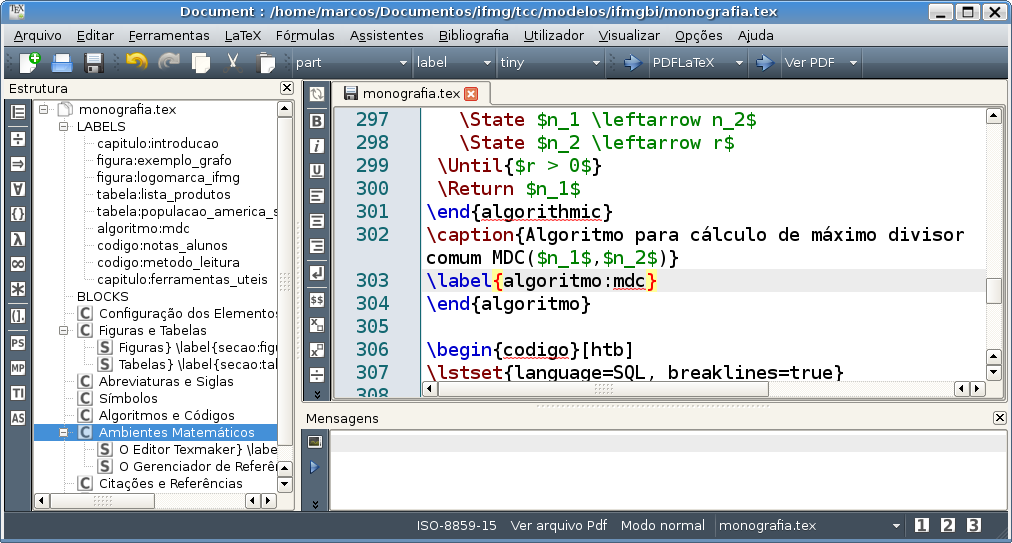
\includegraphics[width=\textwidth]{texmaker.png}
 \fautor
\end{figure}

\begin{figure}[htb]
\caption{Site do ShareLaTeX}
 \label{fig:sharelatex}
 \centering
 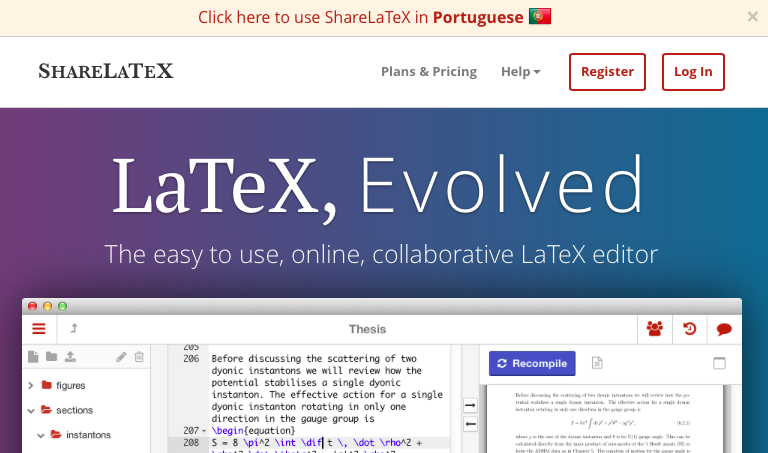
\includegraphics[scale=0.5]{sharelatex.png}
 \fautor
\end{figure}

\begin{figure}[htb]
 \caption{Tela do JabRef}
 \label{fig:jabref}
 \centering
 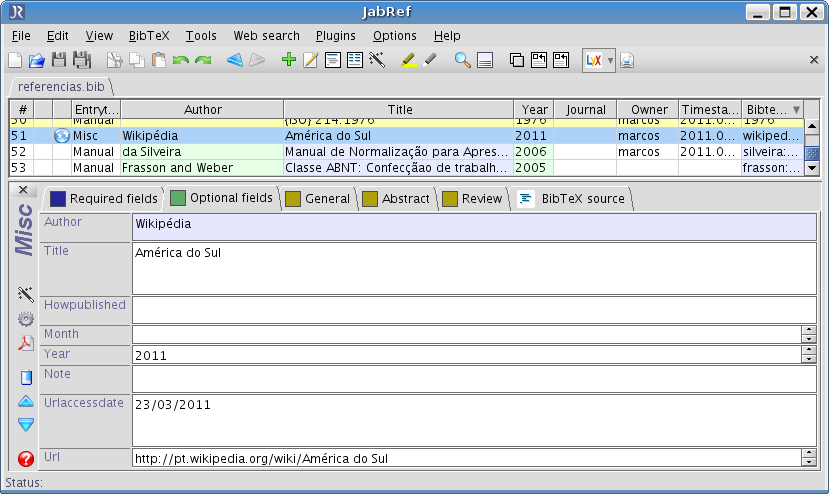
\includegraphics[scale=0.45]{jabref.png}
\fautor
\end{figure}

O Texmaker pode ser obtido em \url{www.xm1math.net/texmaker} e o JabRef pode ser obtido em \url{jabref.sourceforge.ne}. É importante ressaltar que o Texmaker é apenas um editor, para compilar os documentos é necessário um ambiente \LaTeX instalado. Os ambientes Latex mais populares são o Texlive (\url{www.tug.org/texlive}) e o MiKTex (\url{miktex.org}). 

As estrutura de referências do bibtex utilizadas nesse \textit{template} contém alguns parâmetros adicionais que o modelo geral não tem, conforme pode ser consultado em \citeonline{abntex2cite-alf}. Desta forma, recomenda-se fortemente o uso do gerenciador de referências JabRef, uma vez que é possível customizá-lo para atender estas exigências. O código de customização pode ser visto no \autoref{chapter:configuracao-jabref}.

O ShareLaTeX é uma ferramenta de edição de documento em \LaTeX de forma online e está disponível em \url{www.sharelatex.com}. A ferramenta permite o compartilhamento e edição simultânea do conteúdo. Além disso, pode-se consultar o histórico da edições realizadas no documento. A principal vantagem de utilizar o ShareLaTeX é não precisar instalar o compilador para LaTeX.
%
%\chapter{Citações e referências}
%\label{chapter:citacoes}
%

Em documentos acadêmicos podem existir as citações podem ser: \textbf{implícitas} quando as referências não fazem parte do texto ou \textbf{explícitas} quando o autor referente a citação é mencionado explicitamente na sentença. Nesse sentido, deve-se utilizar os comandos específicos para cada tipo de citação, ou seja, em citações explicitas deve-se usar o comando \comando{citeonline\{\}} e nas demais situações é usado o comando \comando{cite\{\}}. Alguns exemplos são apresentados no \autoref{qua:exemplo-citacao}.

\begin{quadro}[htb]
\caption{Exemplos de citações no documento}
\label{qua:exemplo-citacao}
\centering\small 
\begin{tabular}{|c|c|}        \hline
\textbf{Código em \LaTeX} & \textbf{Código Compilado}\\ \hline\hline
\begin{minipage}[t]{\VerbL}
\vspace{5pt}
\begin{verbatim}
A ironia será assim uma ... proposta
por \citeonline{10520:2000:4.1-1}.
\end{verbatim}
\vspace{5pt}
\end{minipage}
&
\begin{minipage}[t]{\LatL}
\vspace{5pt}
A ironia será assim uma ... proposta 
por \citeonline{10520:2000:4.1-1}.
\vspace{5pt}
\end{minipage}\\\hline

\begin{minipage}[t]{\VerbL}
\vspace{5pt}
\begin{verbatim}
\citeonline[p.~146]{10520:2000:4.2-2}
dizem que ... 
\end{verbatim}
\vspace{5pt}
\end{minipage}
&
\begin{minipage}[t]{\LatL}
\vspace{5pt}
\citeonline[p.~146]{10520:2000:4.2-2} dizem que {...}
\vspace{5pt}
\end{minipage}\\ \hline

\begin{minipage}[t]{\VerbL}
\vspace{5pt}
\begin{verbatim}
``Apesar das ... da filosofia''
\cite[p.~293]{10520:2000:4.1-2}.
\end{verbatim}
\vspace{5pt}
\end{minipage}
&
\begin{minipage}[t]{\LatL}
\vspace{5pt}
``Apesar das {...} da filosofia'' \cite[p.~293]{10520:2000:4.1-2}.
\vspace{5pt}
\end{minipage} \\ \hline

\begin{minipage}[t]{\VerbL}
\vspace{5pt}
\begin{verbatim}
Depois, ...  que prefiro
\cite{10520:2000:4.1-3}.
\end{verbatim}
\vspace{5pt}
\end{minipage}
&
\begin{minipage}[t]{\LatL}
\vspace{5pt}
Depois, {...} que prefiro \cite{10520:2000:4.1-3}.
\vspace{5pt}
\end{minipage}\\ \hline

\end{tabular}
\end{quadro}


Para especificar a página, seção ou capítulo consultado na referência é preciso acrescentá-lo entre colchetes com os comandos \comando{cite[página]\{\}} ou \comando{citeonline[página]\{\}}. O texto colocado entre colchetes aparecerá logo após o ano. Maiores informações sobre os comandos utilizados para citação posem ser consultados no manual de referência da abnTeX2, incluindo o uso de \textbf{apud} \cite{abntex2cite-alf}.


\section{Citações Indiretas}

As citações indiretas são caracterizadas como uma espécie de paráfrase das ideias de um determinado autor, ou seja, o pesquisador, por meio de suas próprias palavras, interpreta o discurso de outrem, contudo, mantendo o mesmo sentido. Outro aspecto que deve ser considerado é a necessidade de o autor (ou os autores) e o ano em que a obra foi publicada serem mencionados. 

Nas citações indiretas há duas formatações possíveis dependendo de como ocorre a citação no texto. Quando o autor é mencionado explicitamente utiliza-se o comando \comando{citeonline\{\}}, caso contrário, deve utilizar o comando \comando{cite\{\}}. 



\section{Citações diretas}
\label{sec-citacao}


As citações diretas ocorrem quando o texto de uma referência é transcrito literalmente. As citações diretas curtas (até três linhas) são inseridas no texto entre aspas duplas. As aspas simples são utilizadas para indicar citação no interior da citação: \aspas{Nas citações, as chamadas pelo sobrenome do autor [...] incluído na sentença devem ser em letras maiúsculas e minúsculas e, quando estiverem entre parênteses, devem ser em letras maiúsculas} \cite[sec.~5]{NBR10520:2002}.

\begin{verbatim}
``Nas citações, as chamadas pelo sobrenome do autor [...] incluído na 
sentença devem ser em letras maiúsculas e minúsculas e, quando 
estiverem entre parênteses, devem ser em letras maiúsculas''
\cite[5]{NBR10520:2002}.
\end{verbatim}

Cabe ressaltar que em \LaTeX as aspas iniciais são diferentes das finais. Para tanto, pode-se utilizar o comando \comando{aspas\{CONTEUDO\}} para inserir um determinado conteúdo entre aspas.

As citações diretas longas (com mais de 3 linhas) podem ser inseridas por meio do ambiente \texttt{citacao}:

\begin{citacao}
As citações diretas, no texto, com mais de três linhas, devem ser
destacadas com recuo de 4 cm da margem esquerda, com letra menor que a do texto
utilizado e sem as aspas. No caso de documentos datilografados, deve-se
observar apenas o recuo \cite[5.3]{NBR10520:2002}.
\end{citacao}

Use o ambiente assim:

\begin{verbatim}
\begin{citacao}
As citações diretas, no texto, com mais de três linhas [...] deve-se 
observar apenas o recuo \cite[5.3]{NBR10520:2002}.
\end{citacao}
\end{verbatim}

O ambiente \texttt{citacao} pode receber como parâmetro opcional um nome de
idioma previamente carregado nas opções da classe (\autoref{sec-hifenizacao}). Nesse
caso, o texto da citação é automaticamente escrito em itálico e a hifenização é
ajustada para o idioma selecionado na opção do ambiente. Por exemplo:

\begin{verbatim}
\begin{citacao}[english]
Text in English language in italic with correct hyphenation.
\end{citacao}
\end{verbatim}

Tem como resultado:

\begin{citacao}[english]
Text in English language in italic with correct hyphenation.
\end{citacao}


\chapter{Introdução} \label{chapter:intro}

Atualmente as atividades de trânsito, o transporte de mercadorias e de passageiros, são importantes no dia a dia das pessoas e são essenciais para o desenvolvimento humano. Na execução destas atividades, a direção é um dos fatores mais agravantes com a segurança no trânsito. Assim é importante um meio que ofereça suporte ao motorista e propicie uma maior segurança nas rodovias \cite{Fuentes-2011}.

Nesse contexto surgiram as \textit{Vehicular Ad hoc NETworks} (VANETs), um tipo específico de rede \textit{ad hoc} que tem por objetivo dar suporte ao motorista aumentando a segurança, o conforto e a eficiência no trânsito. Veículos pertencentes a uma VANET podem se comunicar entre si ou com equipamentos na margem da estrada e assim trocar dados ou informações \cite{chen-2010}.

A infraestrutura de transporte está saturada devido ao crescente número de veículos, o que resulta em vários problemas (e.g., congestionamentos). Problemas que motivaram pesquisas na área de Sistemas de Transporte Inteligente (\textit{Intelligent Transportation Systems} - ITS). Os ITS em conjuntos com as VANETs buscam otimizar o sistema de transporte, para tal utilizam das redes de comunicação \cite{Figueiredo-2001}. Para comunicar-se no ambiente das VANETs é necessário lidar com os problemas da conexão intermitente e com o pouco tempo dentro da área de comunicação com outros veículos, fatores que podem comprometer a eficiência da comunicação \cite{Rubinstein-2009}.

A partir da comunicação nas VANETs foi possível criar aplicações, que podem ser divididas em duas categorias: aplicações de segurança (\textit{safety applications}), que tem por objetivo propiciar uma maior segurança no trânsito e as aplicações de gerenciamento do tráfego e entretenimento (\textit{non-safety applications}), que tem por objetivo disponibilizar informações do trânsito e propiciar um maior conforto durante a viagem \cite{Soomro-2010}.

Muitas aplicações em VANETs tem por base o \textit{Beaconing}, sendo definido pelo o envio de \textit{beacons} periodicamente. \textit{Beaconing} é uma forma de comunicação utilizada para enviar informações de estado (\textit{status}) do veículo e curtas mensagens \cite{noori-2013,Nguyen-2002}.

Para avaliar o desempenho de novos protocolos, aplicações e arquiteturas é necessário a execução de experimentos. No ambiente das VANETs, a execução de experimentos no mundo real geralmente são difíceis e podem ter um alto custo envolvido. Nesse âmbito a simulação é um método eficaz, por possibilitar a avaliação de desempenho de maneira mais fácil e barata através de um ambiente simulado. Entretanto, é importante o uso de um modelo de mobilidade realista, para que assim os resultados da avaliação façam uma previsão precisa de como será o desempenho no mundo real \cite{Mahajan-2006,Saha-2004}.

Na literatura existe uma variedade de protocolos de roteamento para VANETs, sendo separados por paradigmas utilizados e geralmente para um cenário específico. Os protocolos devem ser robustos ao ponto de conseguir lidar com a alta mobilidade dos veículos e conseguir enviar e receber de mensagens entre os veículos e a infraestrutura na margem da estrada \cite{Alves-2009}. Uma abordagem para o roteamento das mensagens utiliza os encontros (encontros oportunistas) entre veículos para transmitir as mensagens. Ao enviar uma mensagem esses protocolos é necessário decidir para qual veículo enviar a mensagem e assim decidir se determinado veículo é um bom nó para conduzir determinada mensagem, para isto levam em conta a mobilidade dos veículos \cite{costa-2013}.

Com a crescente quantidade de veículos nas rodovias é necessário um método de se inferir o padrão de mobilidade dos veículos de modo rápido para tomada de decisão sobre o encaminhamento da mensagens. Nesse âmbito propomos a classificação dos veículos em categorias e a incorporação destas categorias em algum protocolos de roteamento com o intuito de otimizar o encaminhamento de mensagens em VANETs.

O restante deste documento está organizado da seguinte forma: A \autoref{section:objetivos} descreve os objetivos do trabalho e a \autoref{section:motivacao} a motivação; o \autoref{chapter:fundamentos} discorre sobre os conceitos das VANETs e afins; o \autoref{chapter:trabRela} apresenta os trabalhos relacionados; e por fim o \autoref{chapter:metodologia} apresenta as atividades e o cronograma da proposta de trabalho deste projeto.

\section{Objetivos} \label{section:objetivos}

O objetivo geral deste projeto é otimizar o roteamento ou o encaminhamento de mensagens utilizando a classificação dos veículos em categorias para implementação de serviços \textit{non-safety}. Os principais resultados esperados deste projeto:

\begin{itemize}
    \item classificação dos veículos em categorias para tomada de decisão no encaminhamento de mensagens;
    \item Otimizar o encaminhamento de informações no modelo de comunicação veículo com veículo;
    \item criação de cenários, em um ambiente de simulação, para validação dos resultados.
\end{itemize}

\section{Motivação} \label{section:motivacao}

A cada dia aumenta a quantidade de veículos em circulação, fato que pode agravar a caótica situação do trânsito mundial. Entretanto, uma maior quantidade de veículos aumentará a probabilidade de encontros oportunistas e assim as chances de comunicação entre os veículos. Nesse cenário de dezenas ou centenas de veículos em um mesmo local, é necessário um modo rápido de se inferir o padrão de mobilidade dos veículos para ser utilizado na tomada de decisão sobre o encaminhamento de mensagens. Nesse âmbito a classificação de veículos em função dos seus hábitos de mobilidade pode ser uma maneira prática de se inferir o padrão de mobilidade de determinado veículo. Quando for necessário saber o padrão de mobilidade de algum veículo terá apenas que verificar a qual categoria ele pertence. A classificação pode ser utilizada na tomada de decisão se determinado veículo é um bom nó para conduzir determinada mensagem. Também pode ser utilizada para criar mensagens para determinados grupos. Cada grupo sendo composto por uma ou mais categorias. No momento que um veículo receber uma mensagem, ele verifica para quais categorias ela é destinada, se a dele estiver presente, processará a mensagem, caso contrário a descarta, economizando em processamento. Essa classificação será enviada dentro dos \textit{beacons} e incorporada em algum protocolo de roteamento com objetivo de melhorar o encaminhamento de mensagem.

\chapter{Fundamentos} \label{chapter:fundamentos}

Neste capítulo é apresentado o embasamento teórico obtido a partir de uma pesquisa bibliográfica.

\section{Redes tolerantes a atrasos} \label{section:dtn}

Em uma \sigla{DTN}{\textit{Delay Tolerant Network}}, os nós estão conectados de forma intermitente e novos nós de conexão são, em sua maioria, desconhecidos. Um caminho conectando a origem ao destino (fim a fim) é pouco provável que exista. As DTNs são redes sem fios, com alta mobilidade e baixa densidade de nós, o que torna o roteamento nestas redes um problema desafiador. Elas utilizam a estratégia \textit{store-carry-and-forward} para o roteamento das mensagens \cite{Jain-2004, Bulut-2010}.

Na estratégia \textit{store-carry-and-forward} a informação passa por nós intermediários até chegar ao seu destino. Nela o nó armazena a mensagem que for enviar ou que tiver recebido em um \textit{buffer}, ao encontrar com outro nó, avalia se ele é um bom nó para conduzir essa mensagem, se sim, transfere a mensagem para ele. Esse processo se repete até a mensagem chegar ao seu destino ou seu tempo de vida expirar. Se não existir nenhum nó para transmitir a mensagem, ela é armazenada até uma oportunidade de transmissão. A mensagem é armazenada enquanto seu tempo de vida não expirar. Com o advento das DTNs, a estratégia \textit{store-carry-and-forward} tem sido amplamente aplicada para o roteamento de mensagens. \cite{Bulut-2010}.

A ideia inicial das redes tolerantes a atrasos foi motivada pela proposta de desenvolver uma \sigla{IPN}{\textit{Interplanetary} Internet} e melhorar a comunicação interplanetária. A arquitetura foi desenvolvida de modo que pudesse trabalhar com atrasos e pacotes corrompidos, o que ocorria nas comunicações no espaço. Os conceitos da IPN foram adaptados para redes terrestres, motivado pelo pobre desempenho de algumas redes da época (2002), criando assim o termo \textit{Delay Tolerant Network} \cite{Fall-2003,Pond-2013}.

As DTNs passaram a ser utilizadas em locais de conexão ruim, com longas taxas de erros e atrasos, propiciando assim o conceito de redes oportunistas. Nesse cenário, a arquitetura de rede TCP/IP \footnote{\textit{Transmission Control Protocol} / Internet \textit{Protocol}}, comumente utilizada na Internet, não é a ideal, devido as etapas do seu protocolo de comunicação, o TCP. O TCP é um protocolo orientado a conexão, que utiliza mensagens de confirmação para estabelecer a conexão, transmitir os dados e encerrar a conexão. Assim o TCP utiliza muitos recursos da rede e gasta um tempo não disponível para os cenários de redes com atrasos e desconexões frequentes \cite{Tanenbaum-2011,Pond-2013,Fall-2003}.

\section{Redes oportunistas} \label{section:opotunismo}

Usuários da rede mundial de computadores, com inclusão de dispositivos da computação ubíqua buscam estar conectados a todo momento. Em função da mobilidade, esses usuários podem experimentar momentos de falta de cobertura pelas redes. Desse modo, a conexão em conjunto com a mobilidade é de suma importância para esses usuários. A intermitência da conexão é um problema desafiador \cite{Sastry-2009,Sastry-2011,Hui-2005}.

A maioria dos dispositivos móveis atualmente são equipados com Wi-Fi, \textit{Bluetooth}, sensores e outros componentes. Além disto, a maioria dos veículos modernos têm instalado interfaces de comunicação sem fio e vários sensores. O uso generalizado desses dispositivos e veículos cria um grande número de oportunidades de encontros, chamados de encontros oportunistas. As redes oportunistas aproveitam desses encontros oportunistas para efetuar a troca de mensagens. A mobilidade dos nós é o fator chave nas comunicações oportunistas \cite{Khalid-2012}.

Nas redes com infraestrutura, os usuários podem, em função da mobilidade, experimentar momentos de falta de cobertura pelas redes, definido por ilhas de conexão (e.g., Wi-Fi de ``casa'' e do ``trabalho''). Esse problema motivou pesquisas por tecnologias alternativas, mas apesar dos esforços, a população ainda sofre com falta de conexão com a Internet. Para esse cenário, as redes oportunistas são uma tecnologia promissora, onde a informação passa por nós intermediários até chegar ao seu destino, estratégia \textit{store-carry-and-forward} \cite{Pond-2013}.

Nos encontros oportunistas, os dispositivos trocam dados utilizando protocolos de curto alcance a fim de alcançar o destino desejado. Assim, o caminho da origem ao destino é construído ao longo do tempo e consiste de uma cadeia de nós intermediários. Tais nós transportam altruisticamente dados ou mensagens do remetente em vários momentos antes do destino recebê-los \cite{Sastry-2011}.

\begin{figure}[!htbp]
    \centering
    \caption{\label{figure:rote_oport} Ilustração do roteamento oportunista}
    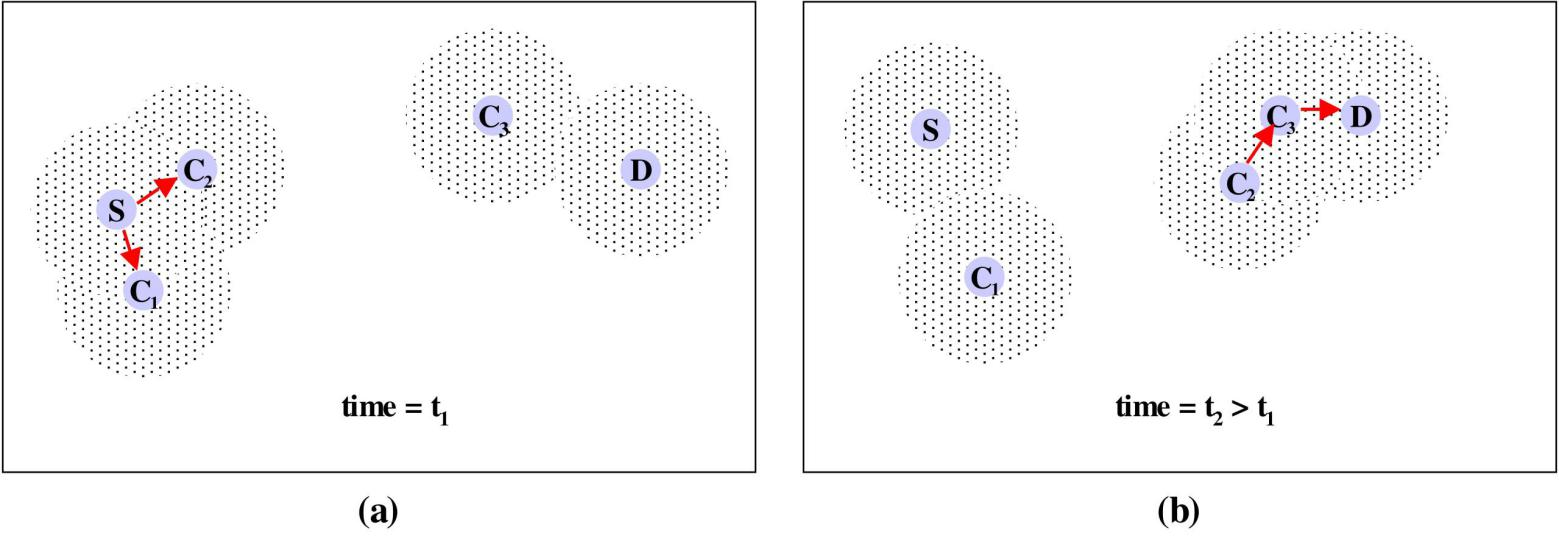
\includegraphics[width=15cm]{img/roteamento.jpeg}
    \legend{Fonte: \cite{Vahdat-2000}}
\end{figure}

O roteamento de mensagens aproveitando-se dos encontros oportunistas é definido como roteamento oportunista, representado na (\autoref{figure:rote_oport}). Na \autoref{figure:rote_oport} (a), um nó fonte $S$ deseja enviar uma mensagem para um nó de destino $D$, entretanto não existe nenhum caminho disponível (i.e., conectividade fim a fim de $S$ para $D$). Assim $S$ transmite sua mensagem para seus dois vizinhos, $C1$ e $C2$, em área de comunicação direta. Algum tempo depois, \autoref{figure:rote_oport} (b), $C2$ entra em alcance de comunicação direta com o nó $C3$ e transmite a mensagem para ele. Por fim, $C3$ tem alcance direto com $D$ e, finalmente, envia a mensagem para o seu destino $D$ \cite{Vahdat-2000}.

\section{Sistemas de transporte inteligente} \label{section:its}

Atualmente a infraestrutura de transporte está saturada, devido ao crescente número de veículos nas últimas cinco décadas, principalmente em áreas urbanas. Acarretando em congestionamentos, acidentes, atrasos no transporte e uma grande quantidade de emissão de poluentes. Esses problemas motivaram pesquisas na área de Sistemas de Transporte Inteligente, do inglês \sigla{ITS}{\textit{Intelligent Transportation Systems}} \cite{Figueiredo-2004}.

Os ITS utilizam a comunicação, os sistemas de informação, o sensoriamento, o processamento de sinais e a tecnologia eletrônica de modo a resolver problemas de transporte (e.g., congestionamentos, falta segurança e pouca eficiência do transporte). Assim tem por objetivo proporcionar segurança, conforto aos passageiros e aumentar a eficiência do tráfego \cite{Figueiredo-2001}.

Os ITS promovem comunicação entre usuário oferecendo condições necessárias para atender aplicações com diferentes requisitos. Um conjunto destas aplicações consiste em um Sistema Inteligente de Transporte, onde seus usuários estão dentro de veículos. O monitoramento cooperativo do tráfego e prevenção de colisões são exemplos destas aplicações \cite{Alves-2009}.

A comunicação entre veículos foi denominada de redes veiculares. Nelas existem as partes sem infraestrutura (\textit{ad hoc}) e com infraestrutura. No início, o termo \textit{Vehicular ad hoc networks} foi criado para se referir apenas a parte \textit{ad hoc}, mas atualmente pesquisadores utilizam este termo para se referir a redes veiculares de modo geral \cite{Yokoyama-2014,Alves-2009,junior-2013}.

\section{Vehicular ad hoc networks} \label{section:VANETs}

A incorporação de tecnologias ubíquas e interfaces de comunicação sem fio em veículos concedeu-lhes a capacidade de se comunicar entre si e com o ambiente em que estão inseridos, o que se convencionou chamar de \sigla{VAN}{\textit{Vehicle Area Network}}. O alcance da comunicação de uma VAN está delimitado a uma certa distância em torno de um veículo que está em movimento. Os dispositivos que estão sobre a cobertura de uma VAN podem estabelecer uma comunicação a fim transmitir dados a qualquer outro dispositivo integrante da rede \cite{Faezipour-2012}.

Nesse contexto está inserido um tipo específico de rede \textit{ad hoc}, as \sigla{VANETs}{\textit{Vehicular Ad hoc NETworks}}. As VANETs são uma subclasse das \sigla{MANETs}{\textit{Mobile Ad hoc NETworks}}, que trocam informações aproveitando os encontros oportunistas (redes oportunistas). O objetivo das VANETs é dar suporte ao motorista, aumentando a segurança no trânsito, o conforto aos passageiros e a eficiência do tráfego \cite{Fuentes-2011}.

Os veículos pertencentes a uma VANET podem se comunicar diretamente entre si, em um modelo veículo com veículo, \sigla{V2V}{\textit{Vehicle-to-Vehicle}}, ou com equipamentos fixos na margem da estrada, \sigla{V2I}{\textit{Vehicle-to-Infrastructure}}, para obter algum serviço ou informação. Tais equipamentos, denominados \sigla{RSU}{\textit{Road Side Unit}}, são localizados ao longo das estradas e são \textit{gateways} entre a infraestrutura e os veículos e vice-versa. As RSUs também podem se comunicar entre si, \sigla{I2I}{\textit{Infrastructure-to-Infrastructure}}, para aprimoramento do controle de sinal. Promover uma comunicação sem fio eficiente para esses modelos é um desafio e uma questão essencial para com os Sistemas de Transporte Inteligente \cite{Faezipour-2012,tangade-2013, Kishimoto-2014}.

Nas VANETs, os veículos são equipados com três dispositivos distintos (\autoref{figure:vanet_car}). Em primeiro lugar são equipados com uma unidade de comunicação \sigla{OBU}{\textit{On-Board Unit}}, que permite a comunicação V2V e V2I. Segundo, um conjunto de sensores (\textit{sensors}) para mensurar o seu próprio estado (e.g., consumo de combustível) e o ambiente (e.g., estrada escorregadia). Esses dados sensoriais podem ser compartilhados com outros veículos de modo a aumentar a consciência na rodovia e assim melhorar a segurança no trânsito. Por fim, um \sigla{TPM}{\textit{Trusted Platform Module}}, dispositivo que oferece armazenamento e computação confiável para os outros dispositivos \cite{Fuentes-2011}.

\begin{figure}[!htbp]
    \centering
    \caption{\label{figure:vanet_car}VANET - modelo simplificado}
    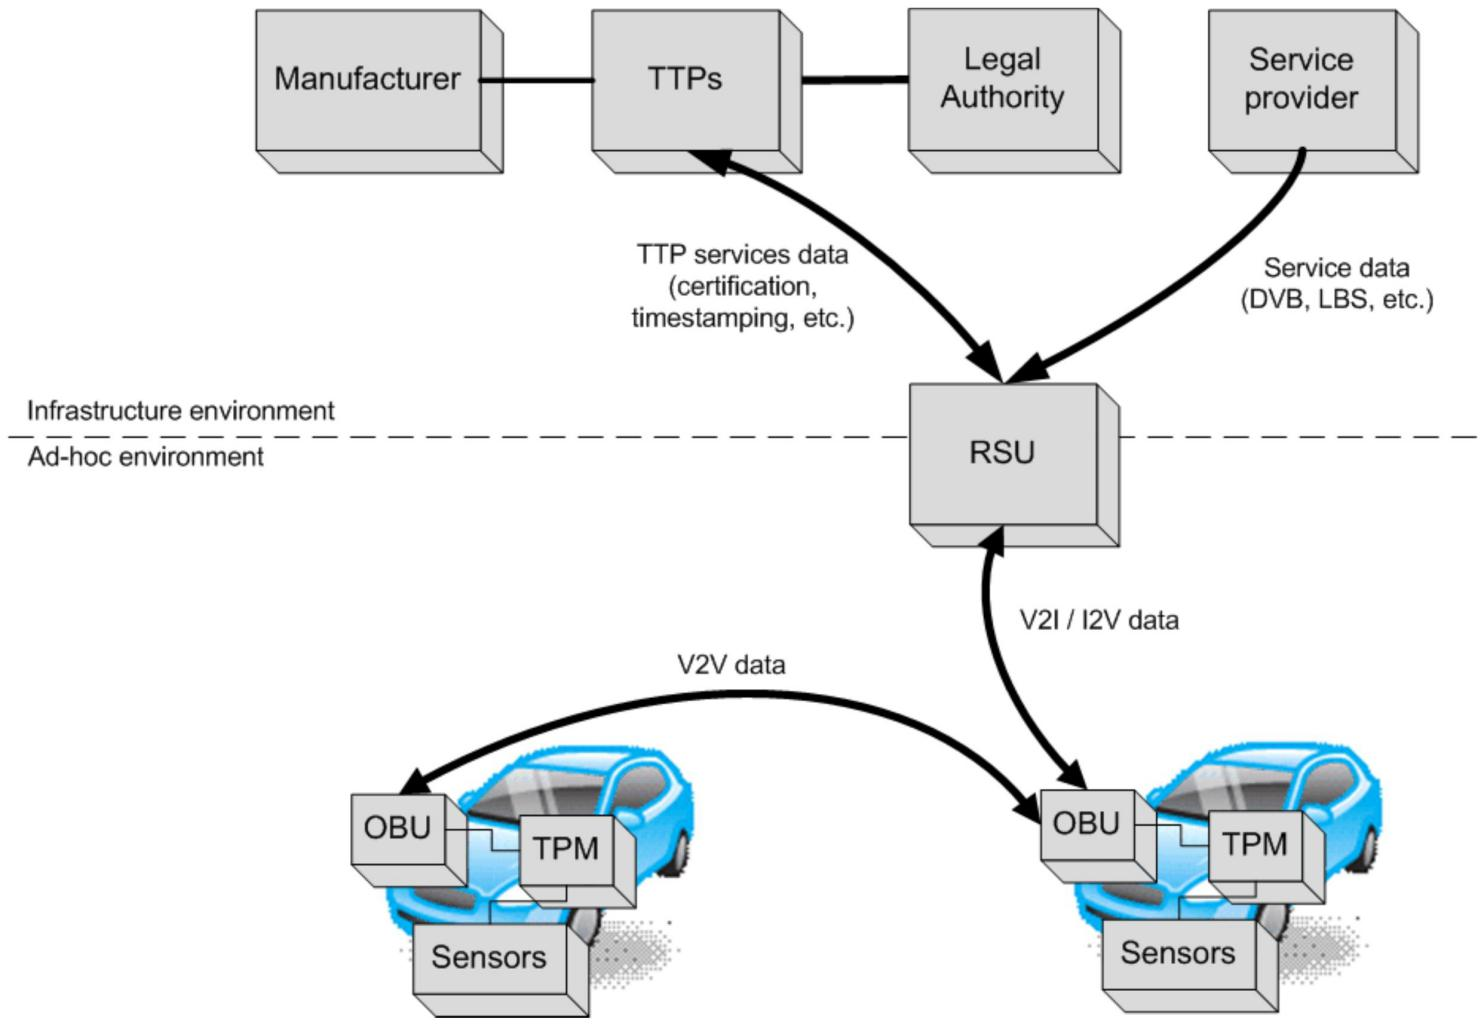
\includegraphics[width=13cm]{img/vanet-car.jpeg}
    \legend{Fonte: \cite{Fuentes-2011}}
\end{figure}

Os fabricantes (\textit{Manufacturers}) são considerados dentro do modelo VANET, por identificarem exclusivamente cada veículo. A autoridade legal (\textit{Legal Authority}) é relacionada a duas tarefas principais, registro de veículos e relatórios de multas. Já os \sigla{TTPs}{\textit{Trusted Third Parties}} oferecem diversos serviços como gerenciamento de credenciais e \textit{timestamping}. Os fabricantes e as autoridades legais estão relacionados com os TTPs por eventualmente precisarem de seus serviços (e.g., para a emissão de credenciais eletrônicas). Os prestadores de serviços (\textit{Service Providers}) oferecem serviços que podem ser acessados através da rede (e.g., serviços baseados em localização) \cite{Fuentes-2011}.

A informação contextual, obtida através dos sensores, pode ser utilizada para melhorar a comunicação e, consequentemente, a qualidade da experiência que os utilizadores podem ter a partir da infraestrutura existente na \sigla{NGN}{\textit{Next Generation Network}}. Uma NGN é essencialmente uma rede baseada em IP que permite que qualquer categoria de clientes receba uma ampla gama de serviços, tais como voz, dados e vídeo através da mesma rede \cite{Dharwadkar-2007}.

O intercâmbio da informação contextual ou dados contextuais demonstra um alto potencial de tornar o sistema de transporte mais seguro (e.g., um assistente do motorista que ajuda na prevenção de acidentes), além de propiciar a troca de informações sobre serviços de pontos de interesse (e.g., receber ofertas de restaurantes que estão ao longo do caminho) \cite{Conti-2010,Mapp-2009}.

Existem algumas questões relacionadas com a troca de dados nas VANETs que ainda carecem de respostas. É necessário, por exemplo, investigar o que um veículo deve transmitir durante os encontros, como compartilhar informações de forma adaptativa e personalizada para usuários específicos, e como embalar os dados para promover a transmissão de forma eficiente, uma vez que os veículos têm pouco tempo dentro da área de comunicação \cite{Faezipour-2012}.

As VANETs têm outras características limitantes, como a velocidade do tráfego, bem como a forma de deslocamento dos veículos, o que pode comprometer a eficácia e a eficiência da comunicação \cite{Rubinstein-2009}. Com tantas informações sendo transmitidas pelas VANETs, também é necessário ter segurança e privacidade durante a comunicação, um cenário amplo de pesquisas \cite{Fuentes-2011}.

\subsection{Dedicated short range communications} \label{subsection:dsrc}

O \sigla{DSRC}{\textit{Dedicated Short Range Communications}} foi desenvolvido para suportar uma variedade de aplicações baseadas na comunicação veicular. O DSRC é um canal de comunicação sem fio de curto alcance projetado especificamente para uso automotivo, com um conjunto correspondente de protocolos e padrões. Tais padrões buscam a interoperabilidade entre dispositivos de diferentes fabricantes. O  DSRC foi desenvolvimento inicialmente para aplicações de prevenção de colisão, aplicações que necessitam trocar dados frequentemente entre os veículos e a infraestrutura rodoviária (RSU) \cite{kenney-2011,Alves-2009}.

Em 1999, a FCC (\textit{Federal Communications Commission}), com um dos primeiros esforços para padronização das redes veiculares nos Estados Unidos, alocou 75 MHz do espectro de frequências na faixa de 5,9 GHz (5,850-5,925 GHz) para aplicações DSRC (\autoref{figure:canais_dsrc}). A faixa é livre, porém licenciada, ou seja, não é cobrado uma taxa pela utilização, mas definem quais as aplicações e tecnologias a serem utilizadas. Em outros países foram definidas outras faixas de frequência \cite{Alves-2009,li-2012,kenney-2011}.

O DSRC foi projetado em um sistema multicanal, com espectro de frequência dividido em sete canais (\autoref{figure:canais_dsrc}). Cada canal tem a largura de banda de 10 MHz, seis deles são definidos como \sigla{SCH}{\textit{Service Channel}} e um como \sigla{CCH}{\textit{Control Channel}}. A faixa de banda 5,850-5,855 GHz é reservada (\textit{guard frequency}). O canal de Controle é utilizado para mensagens de segurança, enquanto os Canais de Serviços são utilizados para aplicações e servições \textit{non-safety} \cite{sattari-2012,li-2012}.

\begin{figure}[!htbp]
    \centering
    \caption{\label{figure:canais_dsrc} Alocação de espectro para aplicações DSRC}
    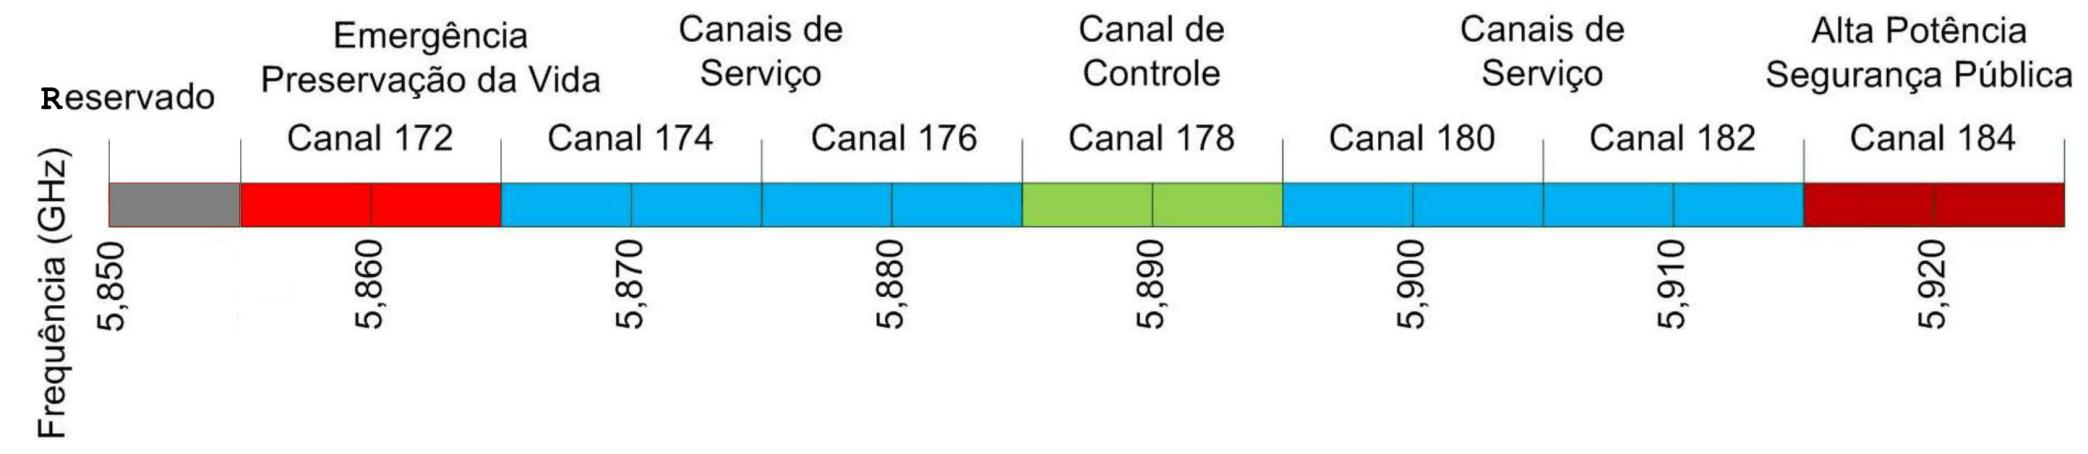
\includegraphics[width=14cm]{img/canais-dsrc2.jpeg}
    \legend{Adapatado de: \cite{Alves-2009}}
\end{figure}

Em 2004, o IEEE \footnote{Institute of Electrical and Electronics Engineers}, inciou a padronização da comunicação em VANETs a partir do IEEE 802.11 (Wi-Fi). Esse padrão é conhecido como IEEE 802.11p \sigla{WAVE}{\textit{Wireless Access in the Vehicular Environment}}. Os documentos: \citeauthor{IEEE-Std-802.11,IEEE-Std-802.11p,IEEE-Std-1609.1,IEEE-Std-1609.2,IEEE-Std-1609.3,IEEE-Std-1609.4}, definem a arquitetura WAVE. O IEEE 802.11p em conjunto com o grupo IEEE 1609 são conhecidos como WAVE, que tem o objetivo de facilitar o acesso à rede no ambiente das redes veiculares \cite{kenney-2011,Alves-2009,sattari-2012,Yokoyama-2014}.

\begin{figure}[!htbp]
    \centering
    \caption{\label{figure:pilha-dsrc-eua} Arquitetura em camadas para comunicação em DSRC nos Estados Unidos}
    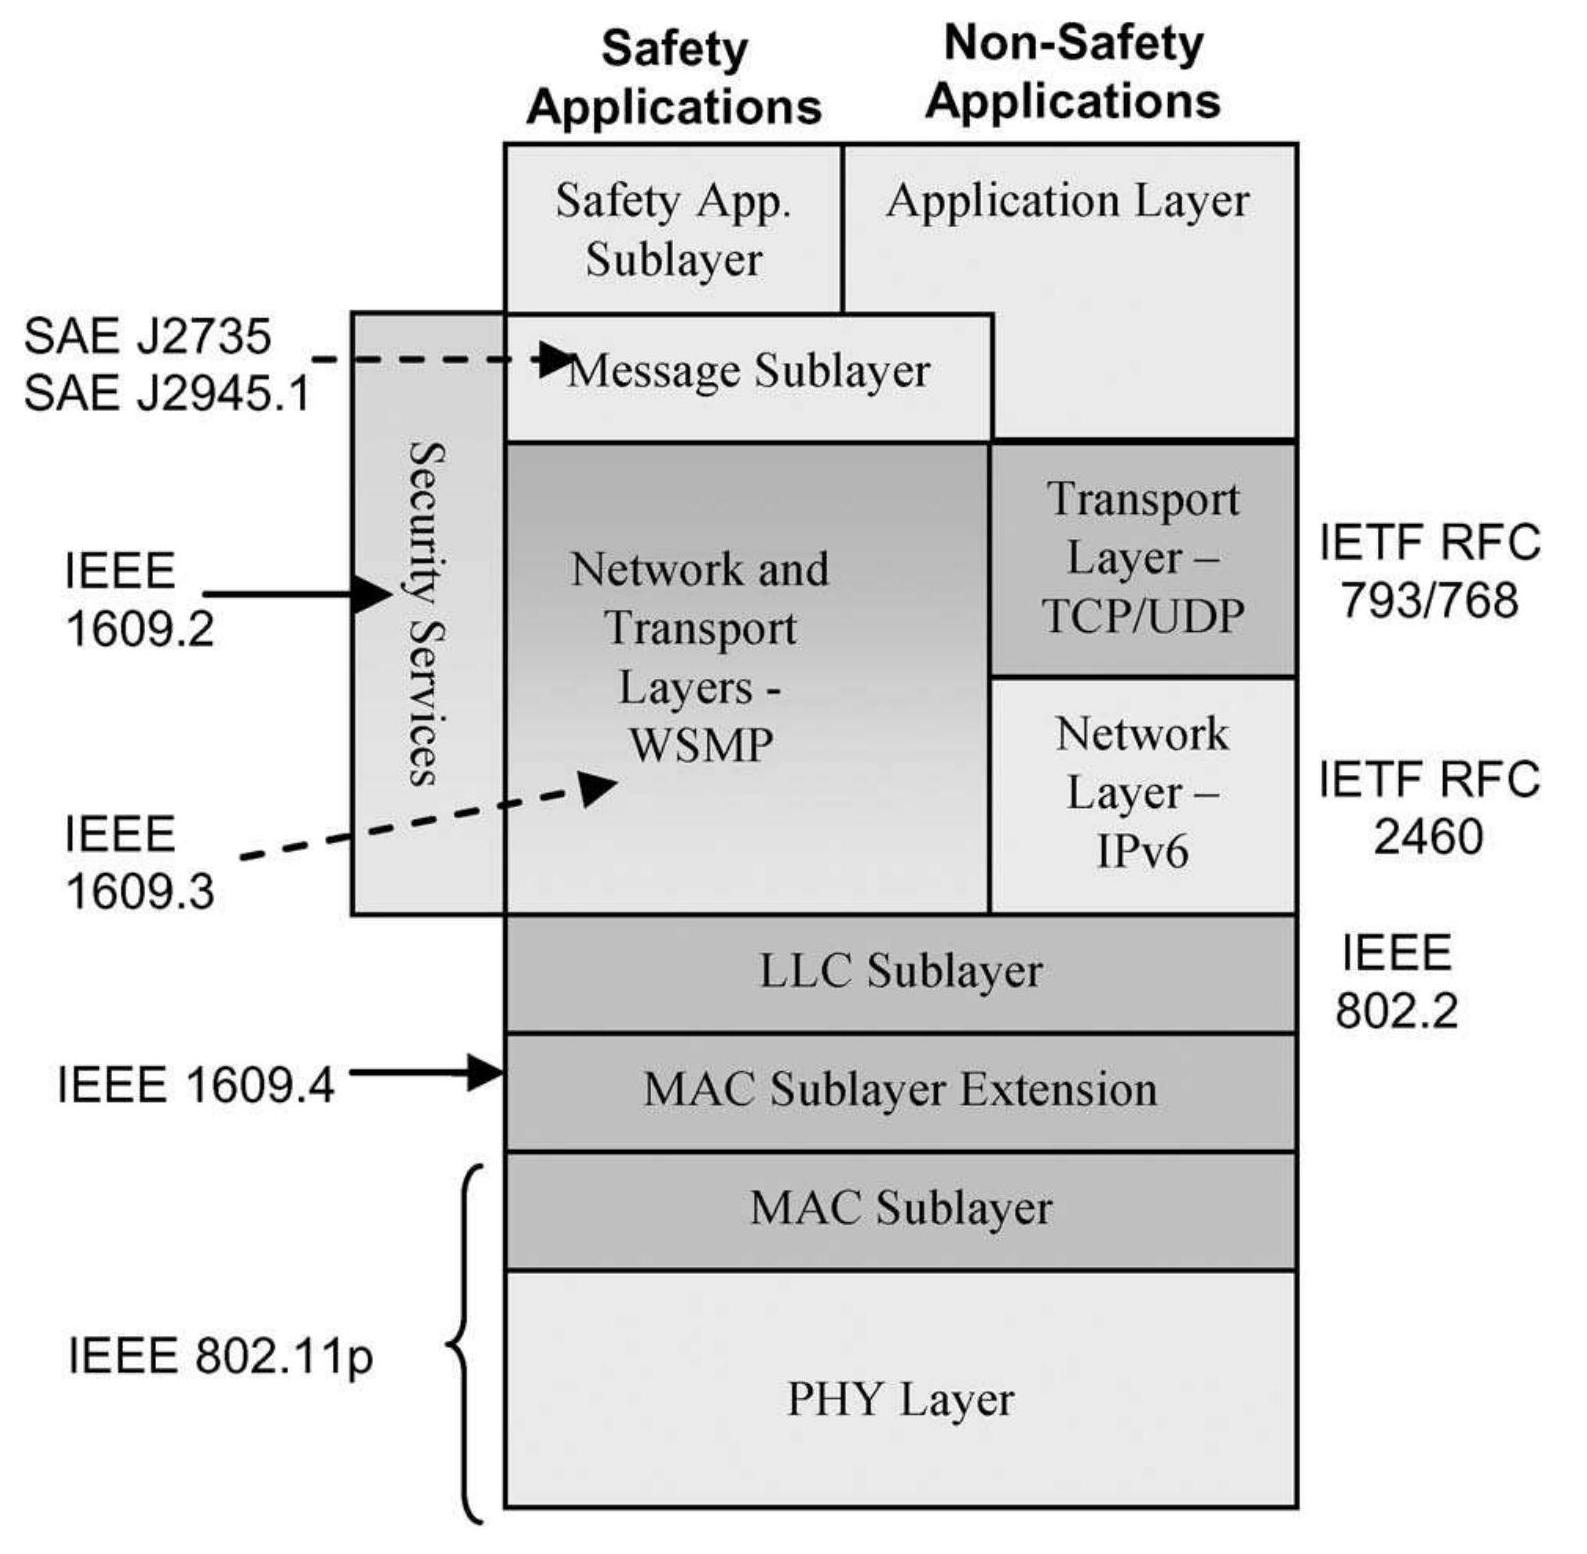
\includegraphics[width=9cm]{img/pilha-dsrc-eua.jpeg}
    \legend{Fonte: \cite{kenney-2011}}
\end{figure}

Na \autoref{figure:pilha-dsrc-eua} pode ser visualizado a pilha de protocolos para comunicação DSRC, com o padrão de protocolos a serem utilizados nas diversas camadas. Para a camada física \footnote{PHY \textit{Layer} ou \textit{Physical Layer}} e a subcamada MAC \footnote{\textit{MAC Sublayer ou Media Access Control}} o DRSC utiliza o IEEE 802.11p. No meio da pilha do DSRC emprega o conjunto de padrões definidos pelo grupo IEEE 1609 \cite{li-2012,kenney-2011}.

O padrão \citeauthor{IEEE-Std-1609.1} especifica serviços e aplicações do gerente de recursos da arquitetura e tem o objetivo de propiciar a interoperabilidade das aplicações WAVE. O padrão \citeauthor{IEEE-Std-1609.2} define o formato das mensagens e o processamento de modo a prover segurança, sendo utilizado para serviços de segurança. O padrão \citeauthor{IEEE-Std-1609.3} define os serviços de rede incluindo o protocolo de mensagens curtas WAVE (\sigla{WSMP}{WAVE \textit{Short Message Protocol}}). O padrão \citeauthor{IEEE-Std-1609.4} define a utilização do Canal de Controle e dos de Serviço \cite{kenney-2011,Alves-2009}.

DSRC suporta alguns dos protocolos de Internet para as camadas de transporte e de rede: o IPv6 \footnote{Internet \textit{Protocol version} 6}, o UDP \footnote{\textit{User Datagram Protocol}} e o TCP. A escolha entre o uso do WSMP ou IPv6 em conjunto com o UDP/TCP depende dos requisitos de cada aplicação. Para mensagens de salto único (\textit{single-hop}), geralmente se utiliza WSMP, por ser eficiente em termos de largura de banda. A transmissão de mensagens de múltiplos saltos (\textit{multi-hop}) pode ser feita utilizando IPv6, mas somente se a transmissão for infraestruturada \cite{kenney-2011}.

O formato das mensagens foi definido pela SAE \footnote{Society of Automotive Engineers} no padrão SAE J2735 \footnote{SAE J2735 DSRC \textit{Message Set Dictionary}} de modo a apoiar a interoperabilidade entre as aplicações DSRC. O SAE J2735 especifica um conjunto de mensagens, elementos de dados (\textit{data elements}) e quadros de dados (\textit{data frame}) para uso nas aplicações DSRC/WAVE \cite{kenney-2011,li-2012,Yokoyama-2014,grilli-2010}.

O SAE J2735 define 15 tipos de mensagens, a maioria delas têm em seu escopo a identificação do veículo, dados de localização e o \textit{timestamp}. Um exemplo destas mensagens é a \sigla{BSM}{\textit{Basic Safety Message}}, que transmite informações sobre o estado (e.g., velocidade e localização) do veículo para veículos próximos. Um elemento de dado é uma informação obtida por algum sensor presente no veículo (e.g., velocidade) e por conceito é indivisível. O agrupamento de um conjunto de elementos de dados forma um quadro de dados. Aliada a SAE J2735, existe a SAE J2945.1 (SAE J2945.1 DSRC Minimum Performance Requirements), ainda em desenvolvimento, que especifica os requisitos mínimos de desempenho das comunicações DRSC definidas pela SAE J2735 \cite{li-2012,grilli-2010,kenney-2011}.

\subsection{Beaconing} \label{subsection:beacons}

Um típico quadro de \textit{beacon} (\textit{frame beacon}), em redes sem fio infraestruturadas é um pequeno quadro, transmitido por difusão (\textit{broadcasting}) periodicamente pelo \sigla{AP}{\textit{Access Point}}, por exemplo a cada 100 ms. Os \textit{beacons} informam a presença de um AP para os clientes e carregam parâmetros do sistema, tais como o identificador do AP, o \textit{timestamp}, quanto tempo até o próximo sinal e as configurações de segurança \cite{Kurose-2012,Tanenbaum-2011}.

No cenário de redes sem fio sem infraestrutura (\textit{ad hoc}), não existe uma infraestrutura (AP) que gerencia as conexões, assim os dispositivos se comunicam em pares, assumindo a responsabilidade pela comunicação e também de enviar os \textit{beacons} quando necessário \cite{Kurose-2012}. A estratégia de utilização de \textit{beacons} para comunicação é definida como \textit{beaconing}. No contexto de VANETs, os \textit{beacons} são utilizados para enviar informações de estado (\textit{status}) do veículo (e.g., velocidade, coordenadas geográficas e aceleração).

De posse das informações de estado dos veículos próximos, é necessário uma aplicação para gerenciá-las e processá-las, apresentando para o motorista avisos importantes sobre a cinemáticas dos veículos próximos. Com esse sistema o motorista pode prever melhor a cinemática dos outros veículos e assim ter uma maior consciência dos acontecimentos e consequentemente propiciar uma maior segurança no trânsito. Os \textit{beacons} são úteis para protocolos de roteamento, pois possibilita a descoberta de um bom veículo próximo para encaminhar uma determinada mensagem  \cite{noori-2013, Nguyen-2002,Fuentes-2011}.

Nas VANETs, os \textit{beacons} precisam ser enviados frequentemente, por serem redes altamente dinâmicas. Entretanto, um frequente envio de \textit{beacons} pode degradar significativamente o desempenho de uma rede altamente densa, devido a muitas colisões de quadros (\textit{frames}). Por outro lado, a baixa taxa de envio de \textit{beacons} pode atrasar a percepção de seus veículos próximos e também reduz a confiabilidade dos protocolos. Desse modo, a frequência ideal de envio dos \textit{beacons} pode variar dependo da quantidade de veículos. \textit{Beaconing} é utilizado em muitas aplicações para VANETs \cite{Nguyen-2002,Thaina-2011,noori-2013}

\subsection{Aplicações em VANETs} \label{subsection:apli_vanets}

As aplicações em VANETs podem ser divididas em duas categorias: aplicações de segurança (\textit{safety applications}) e aplicações de gerenciamento do tráfego e entretenimento(\textit{non-safety applications}). As aplicações de segurança têm como objetivo aumentar a segurança no trânsito e assim proporcionar segurança para os veículos e seus passageiros. Elas requisitam um rígido tempo de comunicação, não tolerando atrasos. Como exemplos destas aplicações temos o assistente para mudança de pista e o sistema de alertas de emergência \cite{aboobaker-2010, al-sultan-2014}.

As aplicações de gerenciamento do tráfego e entretenimento tem objetivo de prover informações do tráfego e melhorar o conforto durante a condução, assim proporcionar uma melhor experiência durante a viagem. Elas não requisitam um rígido tempo de comunicação como as aplicações de segurança. Como exemplos destas aplicações temos o sistema de informação do tráfego, o sistema de avisos de pontos de interesse e o provimento de Internet \cite{Soomro-2010,aboobaker-2010,Yokoyama-2014}.

\subsection{Padrões de mobilidade veicular} \label{subsection:pmv}

A mobilidade é uma espada de dois gumes, por um lado apresenta um problema desafiador em manter a conexão, por outro propicia os encontros oportunistas que podem ser explorados por redes oportunistas. A mobilidade humana é limitada geograficamente pela distância que pode-se viajar dentro de um dia. Ela é moldada por relações sociais, por ser mais propenso visitar lugares onde amigos vivem ou pessoas semelhantes e lugares que já visitou no passado \cite{Cho-2011, Hui-2005}.

As pessoas, geralmente, se movem periodicamente dentro de uma região limitada, mas, ocasionalmente, fazem viagens de longa distância. A probabilidade de uma pessoa deslocar-se até um local distante é maior se nas proximidades desse local ela já tiver algum amigo. Assim a influência da amizade na mobilidade é mais forte do que a influência da mobilidade sobre a criação de novas amizades \cite{Cho-2011}.

As pessoas apresentam um forte comportamento periódico durante certos períodos do dia alternando entre locais primários (e.g., ``casa'') e secundários (e.g., ``trabalho'') nos dias de semana. Para os fins de semana os locais secundários são definidos pelos lugares presentes na vida social de cada pessoa (e.g., um bar) \cite{Cho-2011}. Para um padrão de mobilidade em um contexto veicular é necessário analisar algumas questões, tais como o horário de pico, a mobilidade alcançada em um dia, o desempenho dos veículos na rodovia e a presença de veículos pesados/grandes na rodovia \cite{Resende-2009}.

O movimento dos veículos é limitado pela estrutura rodoviária (delimita locais onde o veículo consegue se locomover), além de se movimentar em função dela (e.g., se tem boas pistas ou não, se tem uma pista ou duas, se tem muitos cruzamentos ou poucos) e das leis de trânsito (e.g., velocidade máxima permitida, regras de condução). Assim a mobilidade veicular está ligada diretamente com a roda. A velocidade de um veículo também é baseada em função da velocidade dos outros veículos presentes na rodovia, podendo aumentar ou diminuir sua velocidade e também alterar a sua rota para evitar congestionamentos \cite{Mahajan-2006}.

Veículos de diferentes tipos apresentam distintos padrões de mobilidade, cada qual com suas peculiaridades. Pode-se classificar os veículos em algumas categorias, tais como táxi, ônibus, veículo particular ou de passeio e veículos pesados (caminhões) para transporte de carga. Os ônibus têm uma cobertura espacial e temporal limitada (e.g., um ônibus que em determinado horário tem como rota vários bairros da cidade e depois volta para a rodoviária). Desse modo, os ônibus movem-se ao longo de rotas fixas durante um determinado período de tempo, o que implica e um forte padrão de mobilidade. O que pode ser muito útil para o roteamento, dado que a mobilidade dos ônibus (nós na rede) é de certa forma previsível. Dada uma área de destino de uma mensagem, os ônibus cujas rotas cruzar com essa área devem ser preferidos para o roteamento da mensagem \cite{Zhang-2014,Zhang-2012}.

O padrão de mobilidade dos táxis é mais diversificado do que o dos ônibus, com uma maior cobertura espacial e temporal. A mobilidade dos táxi é afetada por dois fatores, as demandas dos clientes e os hábitos de condução do motorista (e.g., um táxi tem como destino o centro da cidade, entretanto o motorista não passará pela avenida principal na tentativa de evitar congestionamentos). Se um táxi está ocupado por algum cliente, a mobilidade é determinada, principalmente, pelo destino do cliente. O motorista pode escolher o caminho mais curto ou o com menor congestionamento. Se o táxi não está ocupado, a mobilidade depende dos hábitos de condução do motorista e da sua preferência de lugares para buscar por novos clientes \cite{Zhang-2012,Zhang-2014}.

A mobilidade dos caminhões é determinada, principalmente, pelo destino da carga e pela preferência de rotas do motorista (e.g., um motorista de caminhão tem que entregar mercadorias em outro estado, assim o destino final é o outro estado, mas ele pode escolher por qual rota seguir, com melhor pista ou com menos pedágios). Para os veículos de passeio ou particulares o padrão de mobilidade é bem diversificado, movendo-se para qualquer lugar que o motorista desejar, assim a mobilidade é determinada em função de onde o motorista deseja ir, seja para casa de um amigo ou para o trabalho. Os veículos de passeio têm algumas rotas com destino e horários pré-definidos (e.g., ir para o trabalho, levar as crianças para escola) e outras esporádicas (e.g., visitar um amigo, ir ao supermercado) \cite{Cunha-2014}.

\textcolor{red}{Padrões já desenvolvidos Mahajan-2006}
\ideia{Padrões já desenvolvidos Mahajan-2006}
\duvida{Padrões já desenvolvidos Mahajan-2006}

\subsection{Protocolos de roteamento em VANETs} \label{subsection:algo_rot_vanets}

O roteamento de mensagens nas VANETs é uma tarefa desafiadora devido à alta mobilidade dos veículos.
Existe uma variedade de protocolos para roteamento de mensagens para VANETs. Eles podem ser classificados em: topológicos, geográficos, oportunistas e de disseminação de mensagens \cite{Alves-2009}.

Os protocolos topológicos buscam encontrar a melhor trajetória entre a origem e o destino em função das métricas utilizadas. Eles precisam descobrir e manter as rotas em uma tabela antes de enviar os dados.  A mobilidade dos veículos pode provocar rápidas mudanças na topologia da rede o que torna um desafio manter as rotas atualizadas \cite{sa-2012}.

Nos protocolos geográficos é necessário que os nós tenham algum sistema de localização (e.g., GPS \footnote{\textit{Global Positioning System}}). Esses protocolos buscam prover escalabilidade em ambientes de alta mobilidade, por não ser necessário manter informações sobre as rotas. No roteamento, um nó fonte envia pacotes de dados em direção a localização do destino por múltiplos saltos, para isto o nó necessita conhecer a posição de seus vizinhos, normalmente por \textit{beaconing}, e a posição de destino. Para descobrir a posição do destinatário, comumente se utiliza algum serviço de localização, que através de uma requisições retornam a localização do destinatário, se ele for encontrado \cite{Alves-2009}.

Os protocolos oportunistas seguem os conceitos das redes oportunistas, trocando informações através dos encontros oportunistas e utilizando a estratégia \textit{store-carry-and-forward} para o roteamento de mensagens. Assim são adequados para ambientes com escassez de nós na rede e para cenários que não existam garantias de estabelecimento de caminhos fim a fim entre a origem e o destino \cite{oliveira-2010}.

Os protocolos de disseminação de mensagens transmitem as mensagens por difusão (\textit{broadcast}), diferente dos outros protocolos que são ponto-a-ponto (\textit{unicast}). A disseminação de mensagens é essencial para algumas aplicações, como aplicações de assistência ao motorista que exigem a disseminação das informações sobre as condições das rodovias. Esses protocolos utilizam a estratégia \textit{store-carry-and-forward} para encaminhar as mensagem e não utilizam tabelas de rotas \cite{Alves-2009}.

%Existem duas abordagens para a transmissão das mensagens, a de uma cópia e a de múltiplas cópias. Na abordagem de uma cópia existe apenas uma cópia em toda rede, depois da transmissão da mensagem, ela é apagada do nó fonte. Por outro lado, na abordagem de múltiplas cópias a mensagem não é apagada e pode ser transmitida para outros nós durantes encontros oportunistas. As mensagens encaminhadas pela a abordagem de múltiplas cópias tem maior  probabilidade de chegar ao seu destino, entretanto tem maior gasto de recursos do que a abordagem de uma cópia e sem medidas de controle pode inundar a rede \cite{costa-2013}.

O \textit{Epidemic} é um exemplo dos protocolos de disseminação de mensagens, que se baseia na distribuição transitiva de mensagens. Cada nó mantém um \textit{buffer} consistente de mensagens próprias, bem como de outros nós. Uma tabela de \textit{hash} é utilizada, com uma chave única para cada mensagem e um vetor de \textit{bits} (\textit{summary vector}) indicando quais entradas na tabela estão ocupadas \cite{Vahdat-2000,oliveira-2010}.

Quando dois nós entram em alcance de comunicação, o nó com menor identificador inicia uma sessão (\textit{anti-entropy session}) com o outro nó. Nela os nós trocam seus \textit{summary vector} para determinar quais mensagens armazenadas remotamente não foram vistas pelo nó local. Em seguida cada nó solicita cópias das mensagens que ainda não tinha visto. Ao receber as mensagens o nó tem total autonomia para decidir se aceita ou não a mensagem. O nó pode, por exemplo, recusar mensagens acima de determinado tamanho \cite{Vahdat-2000}.

Para evitar conexões redundantes, cada nó mantém um \textit{cache} de nós que teve contato recentemente. A \textit{anti-entropy session} não é reiniciada com nós que foram contatados dentro um período de tempo determinado. O protocolo de roteamento \textit{Epidemic} tem como objetivo maximizar a taxa de entrega de mensagens, minimizando recursos (e.g., memória e largura de banda de rede) consumidos \cite{Vahdat-2000,oliveira-2010}.

\begin{figure}[!htbp]
    \centering
    \caption{\label{figure:epidemic} Ilustração da troca de mensagens no algoritmo \emph{Epidemic}}
    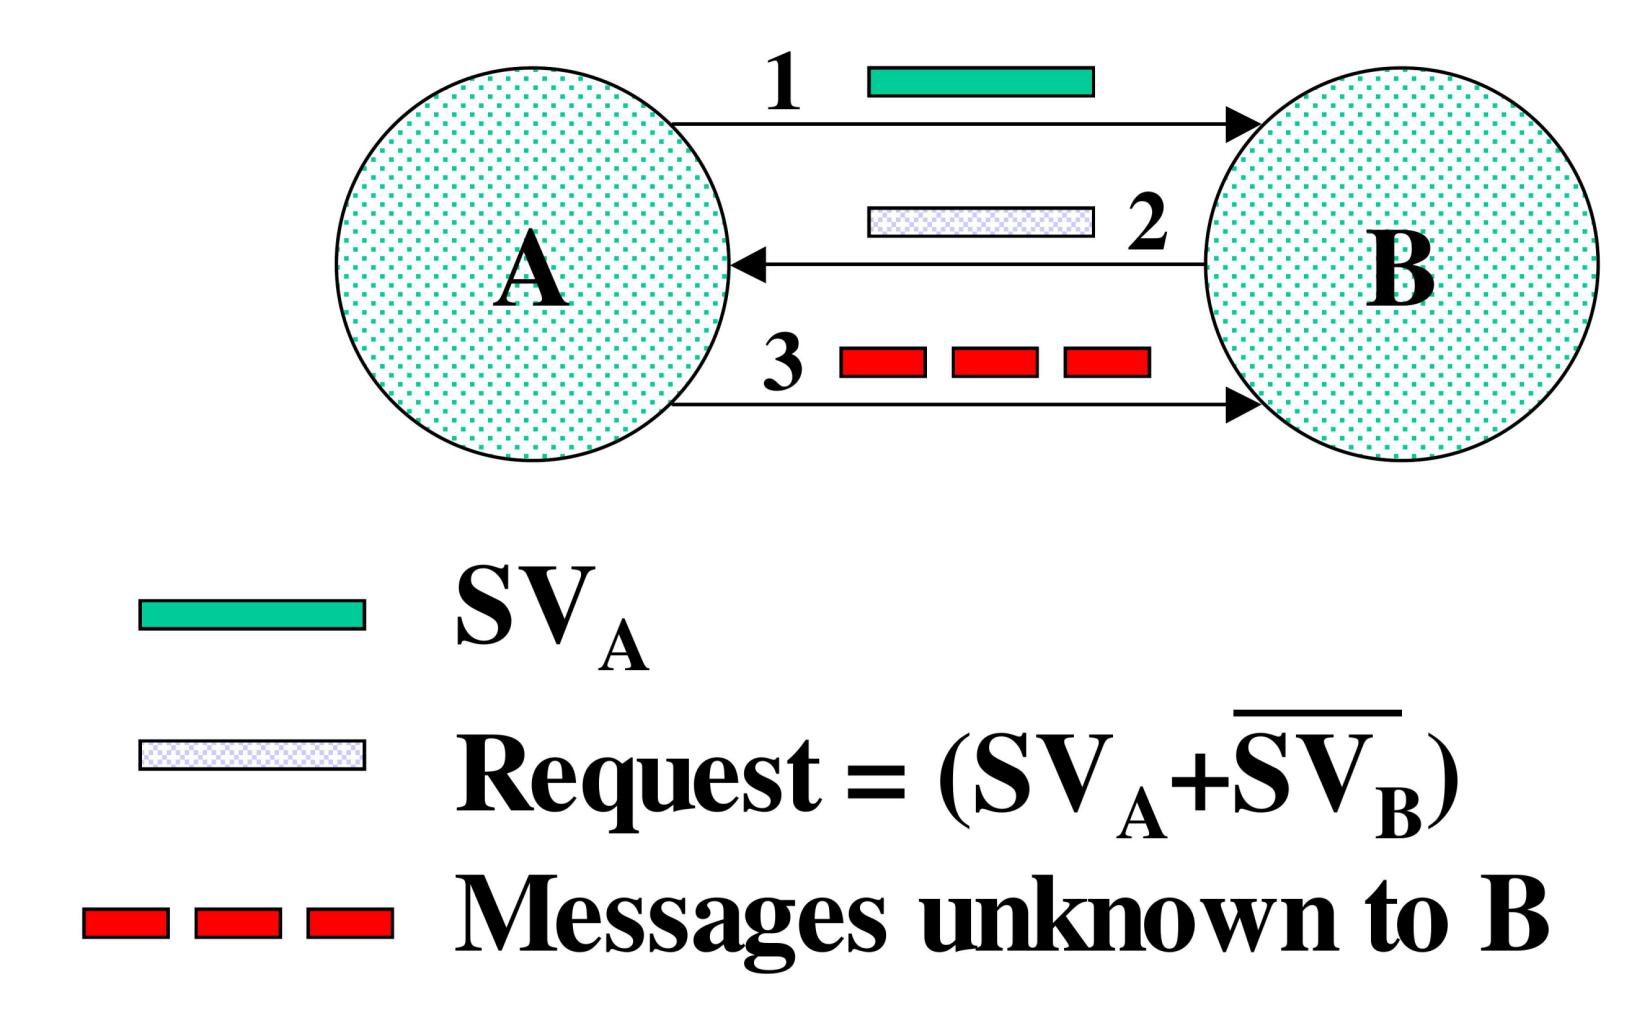
\includegraphics[width=7cm]{img/epidemic.jpeg}
    \legend{Fonte: \cite{Vahdat-2000}}
\end{figure}

Na \autoref{figure:epidemic} pode ser visualizado a troca de mensagens no protocolo de roteamento \textit{Epdemic} do ponto de vista do nó $B$. O nó $A$ entra em contato com nó $B$ e inicia a \textit{anti-entropy session}. No primeiro passo, $A$ transmite seu \textit{summary vector}, SVa para $B$. Em seguida $B$ faz uma operação lógica \textit{AND} entre a negação do seu SVb com SVa que é igual à mensagem que $B$ não ``viu'' ainda presente em $A$. $B$ então solicita essas mensagens para $A$ e por fim $A$ transmite tais mensagens para $B$. Esse processo se repete quando $B$ encontra um novo vizinho.

Como exemplo de protocolo oportunista, temos o \sigla{SKVR}{\textit{Scalable Knowledge-Based Routing}} que utiliza o conhecimento prévio das rotas e horários dos ônibus. Em busca de escalabilidade o SKVR trabalha com dois níveis de hierarquias, o interdomínio (entre rotas de ônibus) e o intradomínio (entre os veículos e uma rota de ônibus). No roteamento intredomínio o algoritmo utiliza o conhecimento prévio das rotas dos ônibus, assim a mensagem é encaminhada para algum veículo que tenha na rota o destino da mensagem ou eventualmente cruze a rota de destino. Em última instância, cópias das mensagens são enviadas para parte dos vizinhos do nó. No encaminhamento intradomínio os nós precisam decidir em que sentido da rota enviar a mensagem. Para isto, uma lista de nós encontrados dentro da rota é armazenada \cite{Alves-2009}.

%\textcolor{red}{add + 2 algoritmos SAR e VADD}

\subsection{Simulações em VANETs} \label{subsection:exp_vanets}

%\textcolor{red}{Titulo: Simulações em VANETs ou Experimentos em VANETs?}

Os experimentos no munto real, dependendo do cenário de estudo, podem ser difíceis e ter um alto custo, como é caso das VANETs. Nesse âmbito a simulação é um método eficaz para a avaliação de arquiteturas e algoritmos de roteamento em VANETs. A simulação é um método mais barato e fácil de utilizar do que a execução dos experimentos no mundo real. Além da possibilidade de replicação dos experimentos de maneira fácil e ser possível isolar algum parâmetro para análise. Entretanto, é importante o uso de um modelo de mobilidade realista para que os resultados da avaliação indiquem corretamente o desempenho real do sistema \cite{Saha-2004,Mahajan-2006}.

A gestão da mobilidade é considerada uma questão crítica em redes de telecomunicação de larga escala. No ambiente veicular, a gestão da mobilidade é ainda mais difícil, devido ao movimento característico dos veículos. Apesar do movimento dos veículos ser restrito a rodovia, eles movimentam-se em altas velocidades, com mudança bruscas na direção do movimento e aceleração, além das variações dinâmicas ao longo do dia \cite{uppoor-2012}.

Nas simulações de tráfego, modelos de mobilidade são utilizados para avaliar o desempenho das aplicações e sistemas de comunicação, permitindo analisar o impacto causado pela mobilidade no funcionamento do sistema. Um modelo de mobilidade representa o movimento dos nós ao longo do tempo, disponibilizando informações de localização, velocidade e aceleração \cite{vieira-2011}.

Os modelos de mobilidade podem ser classificados de a acordo com o nível de detalhe: o macroscópico, o microscópico e o mesoscópico. Do ponto de vista microscópico, a mobilidade de cada veículo é estudada individualmente com a atenção focada na sua performance dentro de todo o sistema de tráfego. Nesse nível é possível modelar várias situações do mundo real, como a mudança de pista e a interação com veículos próximos. Desse modo, são modelos de alta complexidade computacional \cite{vieira-2011,tavares-2013}.

O modelo macroscópico não considerada a mobilidade de um veículo específico, mas o fluxo de veículos e suas características, como velocidade e densidade, assim tem baixa complexidade computacional. O modelo mesoscópico agrega características dos dois outros modelos, buscando a escalabilidade da abordagem macroscópica sem abrir mão dos detalhes da microscópica. Nele as entidades individuas podem ser mapeadas, mas as interações entre elas são abstraídas \cite{tavares-2013,vieira-2011}.

O movimento dos veículos nas simulações é obtido através de algum modelo de mobilidade, como o modelo estocástico, onde o movimento dos veículos é definido como aleatório sobre um grafo \cite{vieira-2011}. Uma maneira de se obter o movimento dos veículos nas simulações é utilizando \textit{datasets} como entrada em algum simulador de mobilidade. A vantagem dessa abordagem é poder reproduzir o movimento dos veículos o mais realista possível no ambiente simulado. Por outro lado, tem a desvantagem de ser necessário coletar os dados e a veracidade do movimento fica dependente da qualidade dos dados. O tamanho da área de coleta e a duração também são importantes.

%\section{Mobile crowd sensing}
%
%Com o crescente avanço das tecnologias de transmissão e de sensoriamento móvel, principalmente pelo crescente uso e proliferação de telefones inteligentes (\textit{smartphones}), levou a era da Internet das coisas. A Internet das coisas visa o sensoriamento e interligação de vários objetos físicos (dispositivos computacionais) e seus arredores em modelo de identificação único na Internet. A proliferação de dispositivos móveis também possibilitou o surgimento do paradigma \sigla{MCS}{\textit{Mobile Crowd Sensing}}, que aproveita os dispositivos móveis e os sensores presentes neles para coletar dados em larga escala \cite{ma-2014}.
%
%No paradigma MCS, os usuários têm a tarefa de recolher e contribuir com dados e assim possibilitar a existência de várias aplicações, tais como o monitoramento do ambiente urbano, o monitoramento do tráfego e estatísticas de disponibilidade de estacionamento. O MCS tem por base a mobilidade dos usuários e assim a mobilidade humana, que oferece oportunidade de sensoriamento de uma área de cobertura e a transmissão de dados \cite{ma-2014}.
%
%O sensoriamento em MCS pode ser feito de duas maneiras, de modo participativo ou oportunista. O sensoriamento participativo exige que os usuários optem conscientemente para atender às solicitações da aplicação, decidindo quando (\textit{when}), onde (\textit{where}), o que (\textit{what}) e como (\textit{how}) realizar o sensoriamento. Por outro lado, no sensoriamento oportunista o aplicativo pode ser executado em segundo plano e coletar dados sem participação ativa dos usuários \cite{ma-2014}.
%
%A transmissão de dados no paradigma MCS também pode ser realizada de duas maneiras, pela infraestrutura ou de modo oportunista. A transmissão pela infraestrutura considera os usuários enviando os dados do sensoriais através da Internet por redes de telefonia móvel celular. Já a transmissão oportunista permite o encaminhamento dos dados pelos contatos oportunos entre os usuários por meio das conexões intermitentes com comunicações de curto alcance como \textit{Bluetooth} \cite{ma-2014}.
%
%A maioria das aplicações MCS adotam o modelo de transmissão baseado em infraestrutura, entretanto ele não é eficiente para cenários onde a cobertura da rede é ruim ou inexistente ou o acesso à rede é caro. O modelo de transmissão oportunista tem a vantagem de não necessitar de um servidor centralizado ou uma infraestrutura de comunicação e gestão, o que pode reduz a carga de trabalho das redes celulares mais densas, transmitindo os dados por contatos oportunistas \cite{ma-2014}.

\chapter{Trabalhos relacionados} \label{chapter:trabRela}

Neste capítulo são apresentadas as publicações encontradas durante a pesquisa bibliográfica que são mais relacionadas com a proposta deste projeto. \citeonline{campos-2010} fizeram uma análise da mobilidade veicular de ônibus públicos urbanos com o objetivo de investigar características da movimentação dos ônibus. Foram capturados, através de um GPS, 32 registros (\textit{traces}) referente ao movimento de um ônibus durante quase um dia em 15 trajetos na cidade de Muriaé (MG). Os autores afirmam que a definição do movimento dos ônibus possibilitaria melhoras nos protocolos existentes para esse tipo de rede, além de possibilitar o desenvolvimento de modelos de mobilidade mais realistas. Como conclusão afirmam que a maior parte do tempo os ônibus públicos urbanos trafegam entre 10 Km/h e 35 Km/h, com aceleração entre -0,5 m/s$^{2}$ e 0,5 m/s$^{2}$.

\citeonline{mateus-2010} parte do pressuposto que apesar de existirem várias soluções propostas para o problema do roteamento em redes veiculares, nenhuma alcançou desempenho satisfatório em mais de um cenário, como o urbano e o rodoviário. Através de simulações analisaram o impacto da densidade, carga da rede e da mobilidade no desempenho de quatro protocolos de roteamento. Após a conclusão de todos os experimentos, afirmam que o uso de parâmetros de mobilidade para realizar o roteamento é uma característica importante. Com o uso desse parâmetro os erros em rotas tendem a ser menor. Também afirma que os protocolos atuais não estão prontos para serem utilizados no mundo real, sendo necessário melhorias nas métricas. Não é necessário um protocolo específico para cada cenário, mas que os protocolos utilizem as informações da rede, como densidade e número de vizinho para assim ter desempenho satisfatório em mais de um cenário.

\citeonline{uppoor-2012} analisaram o tráfego rodoviário na área metropolitana de Colônia, através do \textit{dataset}\cite{tapas-2014}, com objetivo de extrair características de interesse do ponto de vista de rede. A fim de realizar a análise da mobilidade dos veículos, dividiram o \textit{dataset} em células, identificando cruzamentos com, pelo menos, mil veículos ao longo do dia. A lista resultante é analisada. Apresentaram alguns hábitos de mobilidade encontrados no \textit{dataset}. Ao amanhecer, o tráfego é escasso, com maior densidade no centro da cidade. Das 5 às 6 horas o tráfego cresce rapidamente, mas fica restrito a maiores rodovias. Entre 6 e 7 horas o tráfego se intensifica podendo acarretar em congestionamentos, o que leva os motoristas a procurarem por rotas alternativas e aumenta o tráfego em rodovias secundárias. Após às 8 horas a intensidade do tráfego cai rapidamente. Também analisaram o tempo em que os veículos estão dentro da área de comunicação com outros, tendo como distância cem metros uns dos outros. A grande maioria dos encontros dura apenas alguns segundos (1 s - 15 s) e considerando o tempo necessário para identificar o veículo vizinho e começar a comunicar-se, esses encontros são de difícil utilização pelas aplicações, no entanto também existe os encontros com longa duração, que se forem devidamente identificados podem ser aproveitados para troca de grandes quantidades de dados. Por fim relevam a importância de se utilizar definições de mobilidade realistas para avaliações de soluções de rede em ambientes veiculares, o que representa a dinâmica circulação dos veículos.

%\textcolor{red}{add o de taxi, Zhang-2012,Zhang-2014}

Na literatura existem diversas pesquisas com base na comunicação em VANETs e no desenvolvimento de algoritmos para roteamento de mensagens. Dentro desse contexto, algumas pesquisas estão sendo realizados com foco na mobilidade veicular e no desenvolvimento de modelos mobilidade realistas. Entretanto, não foi encontrado nenhum trabalho que propôs-se a analisar a mobilidade veicular com meta de classificar os veículos em categorias. As pesquisas são mais focadas na criação de modelos de mobilidade realistas para serem utilizados em ambientes de simulação e na construção de protocolos de comunicação. Por outro lado, este projeto busca analisar os hábitos de mobilidade dos veículos e consequentemente dos condutores a fim de classificar a mobilidade dos veículos em algumas categorias básicas. Tais categorias apresentam ser uma maneira prática de se obter a mobilidade de um veículo no momento do encaminhamento de mensagens.

% e em conjunto com a adaptação inserção em algum algoritmo de roteamento tentar otimizar o encaminhamento de mensagens. Assim otimizar o encaminhamento de mensagens ...ter a proposta de fornecer um algoritmo de roteamento de forma eficiente e produtiva, o que se resume este trabalho.
% movimentações veiculares, entretanto não foi encontrado nenhum estudo que classifica-se os veículos em função de sua mobilidade em categorias para tomada de decisão sobre o encaminhamento.

\chapter{Metodologia} \label{chapter:metodologia}

Neste capítulo é apresentada a forma como o trabalho será executado na tentativa de alcançar os objetivos desejados. Através de uma pesquisa bibliográfica, pela literatura e anais de congressos, foi obtido o embasamento teórico sobre as redes veiculares, a sua comunicação e protocolos, que serve como base para todo o desenvolvimento deste projeto.

%\textcolor{red}{Intro e considerações finais?...}
%\textcolor{red}{Escrever mais, obter os dados, especificar, ver dados de carros...}

\section{Considerações inicias}\label{section:propostaTrabalho}

Este trabalho tem como proposta fazer uma classificação dos veículos em função de sua mobilidade. Os diferentes tipos de veículos apresentam diariamente um padrão de mobilidade diversificado entre si. Ônibus com rotas bem definidas, sejam elas municipal ou intermunicipal. Táxis têm um padrão de mobilidade em função das preferências do motorista e do destino de seus clientes. Caminhões que levam mercadorias com rotas definidas de um ponto a outro. Veículos particulares ou de passeio, que apesar de uma mobilidade bem diversificada, tem locais de destino frequentes. O padrão de mobilidade se faz com algumas diferenças para os diversos tipos de veículos. Nesse cenário, o trabalho tem como objetivo disponibilizar uma maneira prática de se obter o padrão de mobilidades dos veículos para ser utilizado na tomada de decisão sobre o encaminhamento de mensagens.

\section{Ambiente dos experimentos} \label{section:ambExp}

No desenvolvimento do projeto utilizaremos \textit{datasets} (conjuntos de dados) para prover a mobilidade veicular ao simulador. De início escolhemos o \textit{dataset} TAPAS \textit{Cologne} \cite{tapas-2014}, com dados coletados do movimento de veículos de uma grande área metropolitana da cidade de Colônia (em inglês \textit{Cologne}), na Alemanha. É realista tanto do posto de vista microscópico quanto do macroscópico. O \textit{dataset} foi gerado através de várias ferramentas de modo a obter todos aspectos específicos necessários para a caracterização do tráfego de veículos. O cenário de simulação TAPAS \textit{Cologne} descreve o tráfego dentro da cidade por 24 horas, porém disponível livremente apenas duas horas. Os dados originais derivam do \sigla{TAPAS}{\textit{Travel and Activity Patterns Simulation}}, um modelo de previsão de transporte que examina a futura demanda no transporte de passageiros \cite{uppoor-2012,tapas-2014}.

Mapas realistas da topologia das rodovias da região Colônia foram extraídos da base de dados \sigla{OSM}{\textit{OpenStreetMap}}. Mapas do OSM disponibilizam informações sobre as principais infraestruturas rodoviárias, como rodovias de diferentes tipos, edifícios e também dados de semáforos. Informações obtidas por uma vasta comunidade de contribuintes. Os dados OSM empregados no \textit{dataset} TAPAS \textit{Cologne} cobrem uma área de 400 km$^{2}$ em torno da aglomeração urbana, incluindo cerca de 4500 km de rodovias \cite{tapas-2014,uppoor-2012}.

O realismo em nível microscópico no \textit{dataset} é concedido por uma representação do comportamento dos condutores individualmente, em termos de aceleração, frenagem e presença de veículos nas proximidades. A mobilidade de baixo nível é simulada pelo \sigla{SUMO}{\textit{Simulation of Urban MObility}} \cite{SUMO-2012}, um simulador de mobilidade urbana e tráfego, de código aberto desenvolvido pelo Centro Aeroespacial Alemão (DLR). O SUMO é utilizado e validado por diversas publicações da comunidade de pesquisa de transporte, sendo um dos mais completos e escaláveis geradores de mobilidade microscópica de código aberto disponível. O \textit{dataset} também é realista do ponto de vista macroscópio, pois reproduz os grandes fluxos de tráfego em toda região metropolitana \cite{uppoor-2012,tapas-2014}.

No ambiente simulado utilizaremos o \sigla{OMNeT++}{\textit{Objective Modular Network Testbed in C++}} \cite{OMNeT++-2014} para simular o ambiente de rede sem fio e o SUMO para simular a mobilidade veicular a partir do \textit{dataset} TAPAS \textit{Cologne}. O mecanismo de acoplamento bidirecional entre a rede e o modelo de mobilidade é fornecido pelo \sigla{Veins}{\textit{Vehicles in Network Simulation}} \cite{Veins-2014}.

O OMNeT++ é uma plataforma simulação escrita em C ++ para eventos discretos. Entretanto é aplicado, principalmente, para simulações de rede devido ao seu \textit{framework} INET, que fornece um conjunto de protocolos de Internet (e. g., IPv4, IPv6, TCP, UDP). A sua estrutura é modular, onde cada módulo pode ser utilizado para produzir entidades (módulos) complexas \cite{OMNeT++-2014}. O Veins é um \textit{framework} de código aberto para a execução de simulações em rede veiculares. Baseia-se em dois simuladores bem estabelecidas: OMNeT++ e o SUMO, onde oferecer um conjunto de modelos para simulação de comunicação entre veículos \cite{Veins-2014}. A escolha destes simuladores tem por base a sua validação na comunidade científica por diversas publicações e pelo conjunto ser capaz de simular todo ambiente necessário para o desenvolvimento deste projeto.

%Outro \textit{dataset} que será utilizado neste projeto foi criado e disponibilizado por \citeonline{chen-2010}. É um \textit{dataset} de dados de postagens (\textit{tweets}) obtidos da ferramenta de rede social \emph{Twitter}. Além das postagens, contém a informação da localização de onde foi efetuada a postagem, obtida por serviços de compartilhamento da localização, como \emph{Foursquare}. O \textit{dataset} foi desenvolvido com o objetivo de prover informações úteis para a determinação de padrões de mobilidade humana. De modo a permitir um \textit{dataset} realista e bem diversificado, onde cada usuário teria uma pequena parcela do \textit{dataset}, foi coletado no máximo 200 postagens para cada usuário. No total o \textit{dataset} contém dados de 224.804 usuários e 22.388.315 postagens, sendo que algumas postagens não contém a informação de localização.

\section{Proposta de trabalho} \label{section:propostaTrab}

Este projeto é parte de um projeto maior, que envolve a extração de informações de contexto de \textit{datasets} de mobilidade (projeto de mestrado de Wellington Domingues) e na elaboração de estratégias para uso de informações de redes sociais para melhorar o encaminhamento (projeto de Doutorado de Douglas Fabiano). Este projeto deverá ser desenvolvido no Laboratório Intermídia do Instituto de Ciências Matemáticas e de Computação (ICMC).

A princípio será feita uma análise da mobilidade veicular com o objetivo de verificar as principais características da mobilidade nos mais variados tipos de veículos. Este estudo busca reunir características encontradas nas diversas publicações feitas na área e condensá-las em função dos tipos de veículos. Também será utilizado o \textit{dataset} TAPAS \textit{Cologne} para analisar a mobilidade veicular.

A escolha entre tipos de veículos deverá possibilitar a distinção de um veículo dos demais, levando em conta as características da mobilidade de cada um. A princípio estipulamos os tipos de veículos em: táxi, ônibus (municipal e intermunicipal), caminhões ou veículos de transporte de cargas e veículos de passeio. Ainda será feita uma análise de outros tipos de veículos, como os de serviços públicos (e.g., polícia, ambulância e correios), para ser inserida na classificação.

Após a escolha dos tipos de veículos em conjunto com o padrão de mobilidade de cada um é possível classificar os veículos em categorias. De início a classificação terá 10 categorias, onde acreditamos que poderá cobrir de modo geral todos os tipos de veículos. Categorias de A até I, onde, por exemplo, a categoria B determina o padrão de mobilidade dos táxis. O envio da classificação foi pensado de modo a necessitar de pouca transferência de dados, de modo que seja rápido. Também deve utilizar a estrutura de comunicação das VANETs já desenvolvida, de modo integrar com as tecnologias já desenvolvidas.

Cada veículo enviará a sua categoria para os veículos vizinhos através dos \textit{beacons}. \textit{Beaconing} foi a maneira escolhida por ser uma maneira rápida de enviar dados a outros veículos e já estar implementada por padrão no ambiente das VANETs. Assim através dos \textit{beacons} o veículo saberá quais são seus vizinhos, a localização deles e a categoria que eles pertencem.

Quando um veículo for enviar uma mensagem, analisará a lista de vizinhos e a categoria que eles pertencem. Baseado no destino da mensagem, o veículo processa qual é a categoria mais recomendada para encaminhar a mensagem. Depois o veículo seleciona os veículos da lista de vizinhos que fazem parte dessa categoria e a partir deste momento uma métrica pode ser utiliza para a escolha do veículo ou dos veículos que encaminharam a mensagem. Se não existir nenhum veículo pertencente a categoria próximo do veículo, pode-se esperar um tempo e tentar novamente ou pode aproveitar o encontro oportunista e encaminhar a mensagem para algum veículo vizinho utilizando alguma métrica.

A partir da classificação é possível a implementação de um algoritmo para transmissão de mensagens para um grupo ou tipos específicos de veículos. Uma mensagem enviada para táxis, por exemplo, teria em seu cabeçalho a sua categoria, B. Os outros veículos, que não são táxis, analisariam o cabeçalho a mensagem e ao verificar que é para a categoria B, já a descartam, economizando em processamento. Nesse âmbito é interessante criar uma categoria de veículos para uso geral, sendo destinada para todos os veículos.

Em sequência é feito o estudo de alguns algoritmos desenvolvidos para VANETs. O estudo dos algoritmos tem como objetivo analisar estratégias e funcionalidades implementadas no encaminhamento de mensagens. Com todas estas informações parte-se para adaptação de um dos algoritmos, que leva em consideração a classificação dos veículos em categorias.

Simulação foi a forma escolhida para testar o algoritmo adaptado, porque testes reais são caros, difíceis e podem ser perigosos. Os simuladores que serão utilizados para este trabalho são o SUMO \cite{SUMO-2012}, o simulador de mobilidade; o OMNeT++ \cite{OMNeT++-2014}, o simulador da rede; e o Veins \cite{Veins-2014}, que é a plataforma de integra os dois simuladores.

A partir do algoritmo adaptado, simulações serão feitas utilizando o \textit{datasets} (e.g., o \textit{dataset} TAPAS Cologne \cite{tapas-2014}) como entrada, com objetivo de manter o movimento dos veículos o mais próximo do real possível. Assim as informações de mobilidades dos veículos (e.g., velocidade, direção e tipo do veículo) serão obtidas através do \textit{dataset}. Com resultados das simulações poderemos verificar a eficiência do algoritmo no encaminhamento de mensagens, comparando a taxa de encaminhamento utilizando a classificação dos veículos e sem ela. O algoritmo será implementado em \textit{software} livre e processado em ambiente Cloud-based do Cloud-USP ou Cloud-ICMC. Durante o projeto trabalharemos em cooperação com o grupo de Nishanth Sastry do \emph{King's College} de Londres. O grupo de Nishanth Sastry tem suas pesquisas concentradas nas estruturas e arquiteturas utilizadas para a divulgação e consumo de conteúdo \textit{online}. O que abrange tanto ao nível de infraestrutura (redes de computadores) quanto ao de pessoas (redes sociais).

%Também utilizaremos o \textit{dataset} de postagens na ferramenta de rede social \emph{Twitter}. A análise desse \textit{dataset} tem por objetivo observar semelhanças entre a mobilidade veicular e humana e interligação entre elas. Em conjunto da \textit{Mobile Crowd Sensing} e sua capacidade de descoberta de conhecimento em função dos sensores presentes nos dispositivos e em função do encaminhamento de mensagens, está análise foca em encontrar os principais \textit{hotspots} da movimentação humana e se também se apresentam na base de dados veicular. Assim busca descobrir quais são as principais localidades que são \textit{hotspots} e que poderia ser bom um destino para o encaminhamento de mensagens, levando em conta que em um \textit{hotspot} é provável que existam muitos veículos. Outro ponto da análise desse \textit{dataset} é na busca de obter hábitos de deslocamento de usuários móveis, tais hábitos que são úteis para o roteamento das mensagens.

\section{Cronograma} \label{section:cronograma}

Para cumprir os objetivos descritos, o plano de pesquisa foi dividido em atividades. Nas atividades incluem tarefas do programa de mestrado e desenvolvimento do projeto proposto. O cronograma de atividades do projeto pode ser visualizado na \autoref{section:cronograma}, onde está definida a duração das principais atividades.

\begin{table}[!htbp]
    \centering
    \caption{Cromograma do projeto divido em faixas de tempo} \label{table:cronograma}
    \begin{tabular}{c|c|c|c|c|c|c|c|c|c|c}
        \hline
        \multirow{2}{*}{Atividade} & \multicolumn{4}{c|}{2014} & \multicolumn{5}{c|}{2015}  & \multicolumn{1}{c}{2016} \\ \cline{2-11}
        & 2-6 & 7 & 8-11 & 12 & 1-2 & 3-4 & 5-7 & 8-10 & 11-12 & 1-2\\ \hline
        A1 & $\bullet$ & & $\bullet$ & & & $\bullet$ & $\bullet$ & & & \\ \hline
        A2 & $\bullet$ & $\bullet$ & $\bullet$ & $\bullet$ & $\bullet$ & $\bullet$ & $\bullet$ & $\bullet$ & & \\ \hline
        A3 & & $\bullet$ & $\bullet$ & $\bullet$ & $\bullet$ & & & & & \\ \hline
        A4 & & & $\bullet$ & $\bullet$ & $\bullet$ & $\bullet$ & & & & \\ \hline
        A5 & & & & $\bullet$ & $\bullet$ & $\bullet$ & & & & \\ \hline
        A6 & & & & & & $\bullet$ & & & & \\ \hline
        A7 & & & & & & $\bullet$ & $\bullet$ & & & \\ \hline
        A8 & & & & & & & $\bullet$ & $\bullet$ & & \\ \hline
        A9 & & & & & & & & & $\bullet$ & \\ \hline
        A10 & & & & & & & & & $\bullet$ & $\bullet$ \\ \hline
    \end{tabular}
    %\fonte{Próprio Autor}
\end{table}%

As atividades são descritas abaixo:
\begin{enumerate}
    \item[A1.] Assistir disciplinas definidas para o período e participar das reuniões do grupo.
    \item[A2.] Pesquisa bibliográfica por meio de livros, artigos, anais de congressos e periódicos, como parte do processo contínuo de embasamento teórico.
    \item[A3.] Escrita da monografia para qualificação.
    \item[A4.] Estudo de padrões de mobilidade veicular e a classificação dos veículos em categorias.
    \item[A5.] Estudo de alguns algoritmos de roteamento desenvolvidos para VANETs.
    \item[A6.] Defesa do Exame Geral de Qualificação.
    \item[A7.] Adaptação de um dos algoritmos de roteamento desenvolvido para VANETs e configuração do ambiente de simulação, que compreende a instalação e configuração dos simuladores.
    \item[A8.] Validação dos resultados por meio das simulações e início da escrita da dissertação.
    \item[A9.] Publicação de resultados, por meio da redação de artigos para eventos e periódicos nacionais e/ou internacionais.
    \item[A10.] Finalização da dissertação e preparação para defesa.
\end{enumerate}

%\chapter{Resultados esperados}

%\textcolor{red}{Não sei se este capítulo é realmente importante para o documento de qualificação, afinal, não dá para concluir nada sem resultados do projeto, concorda? Não sei se é legal também ter um capítulo de 1/2 página. Se achar interessante mantê-lo, talvez seja banca acrescentar uma seção 5.1 chamada resultados esperados. O que acha?}

%Com base na pesquisa bibliográfica realizada e na visualização da situação do trânsito mundial, acreditamos que este projeto tem relevância na tentativa de melhorar esse cenário. A classificação de veículos poderia facilitar a tarefa de obter o padrão de mobilidade dos veículos e ajudar a decidir se ele é um bom nó condutor para determinada mensagem. Essa classificação também pode ser utilizada para a comunicação entre veículos de determinadas categorias, enviando mensagens úteis exclusivamente para eles. Nesse cenário os veículos só precisam analisar o cabeçalho do pacote para verificar se a mensagem é para ele ou não. Com a implementação da classificação poderá melhorar um pouco a caótica situação do trânsito mundial e salvar vidas.

% Finaliza a parte no bookmark do PDF, para que se inicie o bookmark na raiz
\bookmarksetup{startatroot}%

\postextual

\bibliography{references}

\end{document}
